%% =====================================================================
%% CytoBridge — any-modality cervical screening: image + questionnaire.
%% VEGA house style. Compile: ~/tectonic_bin/tectonic.exe -X compile main.tex
%% Needs acmart.cls + ACM-Reference-Format.bst + refs.bib + figures/ beside this file.
%% =====================================================================
\documentclass[sigplan,nonacm,screen]{acmart}
\AtBeginDocument{\providecommand\BibTeX{{Bib\TeX}}}
\settopmatter{printacmref=false}
\renewcommand\footnotetextcopyrightpermission[1]{}

\usepackage{tikz}
\usetikzlibrary{arrows.meta,positioning,shapes.geometric,calc,fit,backgrounds}
\usepackage[most]{tcolorbox}
\usepackage{amsmath}
\usepackage{graphicx}

\tikzset{
  box/.style={draw=black, fill=white, rectangle, rounded corners=1.5pt, align=center,
              inner sep=4pt, minimum height=8mm, font=\footnotesize},
  bigbox/.style={box, line width=1pt, minimum width=22mm, minimum height=11mm},
  small/.style={box, font=\scriptsize, inner sep=3pt},
  dec/.style={draw=black, fill=white, diamond, aspect=2.2, align=center,
              inner sep=1pt, font=\scriptsize, minimum height=9mm},
  fl/.style={-{Stealth[length=2mm]}, thick, black},
  lbl/.style={font=\scriptsize, midway, fill=white, inner sep=1pt},
}
\tcbset{vegabox/.style={enhanced, breakable, boxrule=0.5pt, arc=2pt,
  left=5pt,right=5pt,top=3pt,bottom=3pt,
  fonttitle=\bfseries\small, coltitle=white, colupper=black, colback=white}}
\newtcolorbox{defbox}[1][Definition]{vegabox, colback=blue!4,
  colframe=blue!55!black, colbacktitle=blue!55!black, title={#1}}
\newtcolorbox{exbox}[1][Everyday example]{vegabox, colback=orange!7,
  colframe=orange!72!black, colbacktitle=orange!72!black, title={#1}}
\newtcolorbox{keybox}[1][Key insight]{vegabox, colback=green!6,
  colframe=green!48!black, colbacktitle=green!48!black, title={#1}}
\newtcolorbox{gapbox}[1][Research gap]{vegabox, colback=red!4,
  colframe=red!62!black, colbacktitle=red!62!black, title={#1}}
\setlength{\parskip}{2.5pt plus 1pt minus 1pt}
\setlength{\emergencystretch}{3em}

\begin{document}
\title{CytoBridge: A Calibrated, Any-Modality Framework\\ for Cervical Screening Support}
\subtitle{A B.Sc.\ Thesis}
\author{Sammam Mahdi}
\affiliation{\institution{Department of Computer Science}\city{}\country{}}
\renewcommand{\shortauthors}{Mahdi}

\begin{abstract}
Cervical cancer is largely preventable, but screening relies on scarce expert cytologists. Two data sources
can support screening, and they carry \emph{different, complementary} signals: a Pap-smear image reports
\emph{cytological abnormality}, whereas a patient questionnaire supports a \emph{high-risk HPV infection-risk}
estimate. These sources are almost never collected for the same patient, so a jointly trained multimodal model
cannot be built from paired data. We study whether two \emph{independently} trained experts can instead be
combined at the decision level. We build a cytology expert (an EfficientNet-B0 distilled from an
EfficientNet-B4 teacher) and an HPV-risk expert (a RandomForest model on $n=12{,}634$ women from
NHANES~2003--2016), and combine their calibrated probabilities with three components: CO-PRIOR, a
prior-composition step that re-anchors \emph{each} expert to the deployment prevalence \emph{before} pooling;
an asymmetric combiner; and split-conformal abstention. On its held-out validation split the cytology expert
reaches $0.966$ accuracy / $0.998$ AUROC (five-class); the HPV-risk expert reaches $0.721$ accuracy / $0.688$
AUROC under cross-validation. The purpose of the fusion is \emph{not} to raise discrimination beyond the
stronger single expert---it does not---but to add complementary HPV-risk information, keep the fused
probability calibrated when the local prevalence differs from training, and operate when either modality is
missing. We report each expert's results and the fusion behaviour, and we discuss the domain-shift and
patient-pairing limitations candidly.
\end{abstract}

\begin{CCSXML}
<ccs2012><concept><concept_id>10010147.10010178</concept_id>
<concept_desc>Computing methodologies~Artificial intelligence</concept_desc>
<concept_significance>500</concept_significance></concept>
<concept><concept_id>10010405.10010481</concept_id>
<concept_desc>Applied computing~Health informatics</concept_desc>
<concept_significance>500</concept_significance></concept></ccs2012>
\end{CCSXML}
\ccsdesc[500]{Computing methodologies~Artificial intelligence}
\ccsdesc[500]{Applied computing~Health informatics}
\keywords{cervical screening support, knowledge distillation, calibration, decision-level fusion, HPV risk, conformal prediction}
\maketitle

%% =====================================================================
\section{Introduction}
\subsection{Background for the non-specialist}
\begin{defbox}[What this work does, and does not, predict]
Nearly all cervical cancer is caused by persistent high-risk \emph{human papillomavirus} (HPV)
infection~\cite{walboomers1999}. This work supports \emph{screening}, not diagnosis. It builds two models that
predict \emph{different} endpoints: (i) a cytology model that classifies cervical-cell \emph{morphology}
(later reduced to abnormal/normal), and (ii) a questionnaire model that estimates \emph{high-risk HPV
positivity}. Neither predicts cervical cancer directly; they are complementary screening signals.
\end{defbox}

\begin{exbox}[Two independent lines of evidence]
The two models are best seen as two \emph{independently collected} lines of evidence about the same clinical
question---one morphological, one behavioural/epidemiological. They do not observe the same patient, and they
answer related but distinct questions, so combining them is a problem of pooling heterogeneous evidence rather
than of averaging two opinions on one measurement.
\end{exbox}

Cervical cancer remains a leading cause of cancer death in women despite being preventable~\cite{sung2021},
and expert cytologists are scarce, motivating machine-learning support for both the image read and the
risk estimate.

\subsection{The problem, and why paired data are unavailable}
A standard multimodal model is trained on records that contain \emph{all} modalities for \emph{each} patient.
That option is not available here: public cervical-cytology image datasets and public HPV-risk questionnaire
datasets are collected in different studies and share no patients, and there is no key linking a cell image to
a questionnaire respondent. A jointly trained image$+$questionnaire model therefore cannot be built or
evaluated on real paired data. The practical question this work targets is consequently:

\begin{gapbox}[Gaps this work addresses]
\textbf{G1 --- deployable, explainable cytology.} High-accuracy cervical-cytology classifiers are typically
built on large convolutional backbones~\cite{plissiti2018,tan2019efficientnet}, which strains modest hardware
and gives little insight into \emph{why} a cell is flagged unless paired with post-hoc
explanation~\cite{selvaraju2017}. \emph{Addressed by} a distilled, single-GPU EfficientNet-B0 expert with
calibration and Grad-CAM attribution (\S\ref{sec:imgmethod}, \S\ref{sec:imgres}).\\[3pt]
\textbf{G2 --- a calibrated HPV-risk estimate.} Questionnaire-based HPV-risk models are commonly reported by
accuracy or AUROC alone, without a calibrated probability or a stated operating point~\cite{hu2024nhanes}, yet
a screening flag is only actionable as a well-calibrated probability. \emph{Addressed by} an HPV-risk expert with
isotonic calibration and full per-model reporting (\S\ref{sec:tabmethod}, \S\ref{sec:tabres}).\\[3pt]
\textbf{G3 --- combining evidence without paired data.} With no shared patients and each expert calibrated to
its own base rate, classical opinion pooling~\cite{kittler1998} cannot simply average the two outputs; the
priors must be reconciled~\cite{saerens2002} and uncertain cases handled with a coverage
guarantee~\cite{angelopoulos2023}. \emph{Addressed by} CO-PRIOR re-anchoring, an asymmetric combiner, and
conformal abstention (\S\ref{sec:fusmethod}, \S\ref{sec:fusres}).
\end{gapbox}

\subsection{Research question and hypothesis}
\textbf{RQ.} Can independently trained cytology and questionnaire HPV-risk models be combined at the decision
level to give a calibrated, any-modality screening-support output when patient-level multimodal pairing is
unavailable? \textbf{Hypothesis.} Re-anchoring each expert's prior to the deployment prevalence before an
asymmetric pooling step can combine the two complementary signals and keep the fused probability calibrated
across prevalences, without requiring paired training data---while not necessarily improving discrimination
over the stronger single expert.

\subsection{Contributions and implementation choices}
We separate what is a contribution from what is a standard implementation choice.
\emph{Contributions:}
\begin{itemize}
  \item \textbf{A decision-level framework for unpaired complementary modalities} that combines two
    independently trained experts without any patient-level pairing (\S\ref{sec:fusmethod}).
  \item \textbf{CO-PRIOR}: prior correction applied \emph{independently to each heterogeneous expert before}
    decision-level pooling, so both outputs live on one deployment-prevalence scale (\S\ref{sec:fusmethod}).
  \item \textbf{A calibrated, any-modality operating design}: prevalence re-anchoring, an asymmetric cascade,
    and split-conformal abstention, evaluated for calibration and coverage (\S\ref{sec:fusres}).
\end{itemize}
\emph{Implementation choices} (standard components, reported for completeness): EfficientNet-B4$\to$B0
knowledge distillation for the cytology expert, and a class-weighted RandomForest ensemble for the
HPV-risk expert.

%% =====================================================================
\section{Related Work}
\paragraph{Deep cytology classification.} Convolutional models on single-cell benchmarks such as
SIPaKMeD~\cite{plissiti2018} and the Herlev Pap-smear set~\cite{jantzen2005} report high in-distribution
accuracy; EfficientNet backbones~\cite{tan2019efficientnet} with knowledge distillation~\cite{hinton2015}
yield a compact model, the recipe we adopt for the cytology expert.

\paragraph{Questionnaire HPV-risk models.} Models predicting HPV or cervical outcomes from questionnaire and
demographic variables typically use tree ensembles with class-imbalance handling~\cite{hu2024nhanes}; we
follow this recipe for the HPV-risk expert, using class weights rather than synthetic
oversampling~\cite{chawla2002}, and add explicit probability calibration.

\paragraph{Decision-level fusion and calibration.} Combining independent classifiers by opinion pooling and
the sum/product rules is classical~\cite{kittler1998}. Adjusting a classifier's outputs to a new prior is a
single-classifier procedure~\cite{saerens2002}; CO-PRIOR applies it \emph{per expert before} pooling
heterogeneous, differently-calibrated models. Split-conformal prediction~\cite{angelopoulos2023} supplies the
abstention machinery with a coverage guarantee.

%% =====================================================================
\section{Methodology}\label{sec:method}
\subsection{Problem formulation and notation}\label{sec:problem}
Let $x_{\mathrm{img}}$ be a cervical-cell image and $x_{\mathrm{tab}}$ a questionnaire feature vector. The two
frozen experts produce calibrated posteriors
\begin{equation}\label{eq:experts}
p_{\mathrm{img}}=f_{\mathrm{img}}(x_{\mathrm{img}})\in[0,1],\qquad
p_{\mathrm{tab}}=f_{\mathrm{tab}}(x_{\mathrm{tab}})\in[0,1],
\end{equation}
where $p_{\mathrm{img}}$ is the probability of cytological abnormality and $p_{\mathrm{tab}}$ is the
probability of high-risk HPV positivity. Each expert was calibrated at its own training prevalence
($\pi_{\mathrm{img}},\pi_{\mathrm{tab}}$); the deployment prevalence $\tau$ is declared. Either input may be
absent. The fused output is
\begin{equation}\label{eq:fuse}
p_{\mathrm{fused}}=F\big(p_{\mathrm{img}},p_{\mathrm{tab}},\tau\big),
\end{equation}
and the system returns $p_{\mathrm{fused}}$ with a decision in
$\{\textsc{release},\textsc{defer},\textsc{flag}\}$. \emph{Reading Eq.~\eqref{eq:experts}--\eqref{eq:fuse}:}
the two experts are trained and calibrated separately on disjoint data; $F$ is the decision-level operator
(\S\ref{sec:fusmethod}) that reconciles their priors to $\tau$ and pools them. Figure~\ref{fig:arch} shows the
end-to-end system.

\begin{figure*}[t]\centering
\resizebox{0.96\textwidth}{!}{%
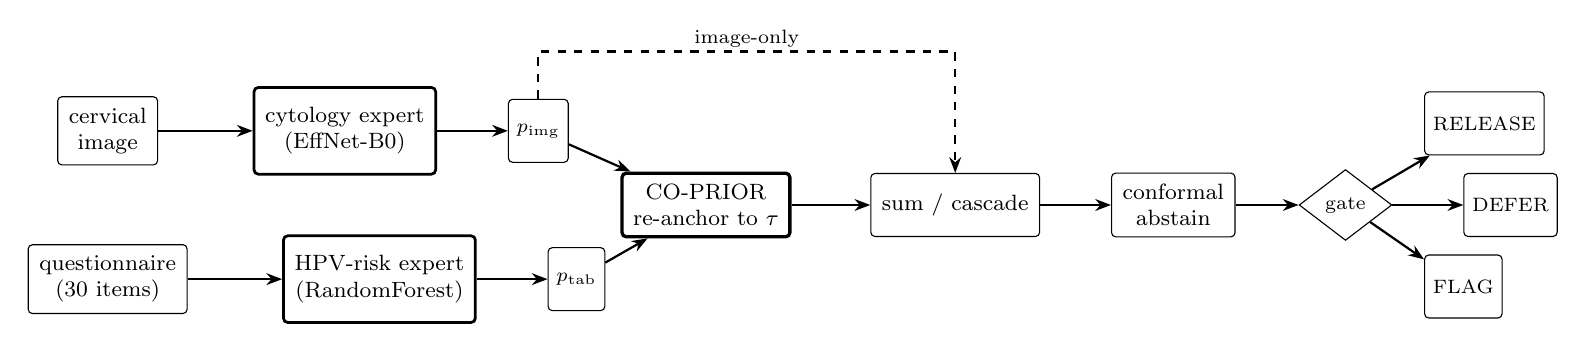
\begin{tikzpicture}[node distance=8mm]
  \node[box] (img) {cervical\\image};
  \node[box, below=10mm of img] (q) {questionnaire\\(30 items)};
  \node[bigbox, right=12mm of img] (imgE) {cytology expert\\(EffNet-B0)};
  \node[bigbox, right=12mm of q] (tabE) {HPV-risk expert\\(RandomForest)};
  \node[small, right=9mm of imgE] (pi) {$p_{\mathrm{img}}$};
  \node[small, right=9mm of tabE] (pt) {$p_{\mathrm{tab}}$};
  \node[box, line width=1.2pt, right=8mm of $(pi)!0.5!(pt)$] (co) {CO-PRIOR\\re-anchor to $\tau$};
  \node[box, right=10mm of co] (comb) {sum / cascade};
  \node[box, right=9mm of comb] (conf) {conformal\\abstain};
  \node[dec, right=8mm of conf] (gate) {gate};
  \node[small, above right=4mm and 7mm of gate] (rel) {RELEASE};
  \node[small, right=9mm of gate] (def) {DEFER};
  \node[small, below right=4mm and 7mm of gate] (flag) {FLAG};
  \draw[fl](img)--(imgE); \draw[fl](q)--(tabE);
  \draw[fl](imgE)--(pi); \draw[fl](tabE)--(pt);
  \draw[fl](pi)--(co); \draw[fl](pt)--(co);
  \draw[fl](co)--(comb); \draw[fl](comb)--(conf); \draw[fl](conf)--(gate);
  \draw[fl](gate)--(rel); \draw[fl](gate)--(def); \draw[fl](gate)--(flag);
  \draw[fl,dashed](pi.north) -- ++(0,6mm) -| node[lbl,pos=0.25,above]{\scriptsize image-only} (comb.north);
\end{tikzpicture}}
\caption{End-to-end system. Two independently trained experts predict different endpoints (cytological
abnormality; high-risk HPV positivity); CO-PRIOR re-anchors each to the deployment prevalence $\tau$ before
the combiner; a conformal check and gate produce RELEASE/DEFER/FLAG. A missing modality bypasses the combiner.}
\Description{Block diagram of the two-expert decision-level fusion pipeline.}
\label{fig:arch}
\end{figure*}

%% ---------------- IMAGE EXPERT METHOD ----------------
\subsection{Cytology expert}\label{sec:imgmethod}
\paragraph{Dataset.} SIPaKMeD~\cite{plissiti2018} contains $5{,}015$ Pap-smear images ($4{,}049$ isolated
single cells and $966$ cluster crops) in five morphology classes: Dyskeratotic, Koilocytotic, Metaplastic,
Parabasal, Superficial--Intermediate. The classes are near-balanced (largest-to-smallest ratio $1.19$). The
first two are the abnormal classes; koilocytosis is a morphological correlate of HPV infection.

\paragraph{Pre-processing.} Images are resized to $380\times380$. Training images receive random horizontal
and vertical flips ($p=0.5$ each), random rotation ($\pm72^{\circ}$), and scale jitter ($0.9$--$1.1\times$),
then ImageNet normalisation; validation images are only resized and normalised.

\paragraph{Knowledge distillation.} An EfficientNet-B4 teacher~\cite{tan2019efficientnet} is distilled into an
EfficientNet-B0 student~\cite{hinton2015}. Schedule: teacher stage~1 (backbone frozen, head only, $30$ epochs,
lr $10^{-3}$); teacher stage~2 (full fine-tune, $50$ epochs, lr $10^{-5}$, \texttt{ReduceLROnPlateau} factor
$0.3$, early stopping); student ($40$ epochs, lr $5\times10^{-5}$, dropout $0.3$, temperature $T=4.0$,
$\alpha=0.1$), batch size $32$, BF16. The distillation loss is
\begin{equation}\label{eq:kd}
\mathcal{L}=\alpha\,\mathrm{CE}\!\big(y,\sigma(z_s)\big)+(1-\alpha)\,T^2\,\mathrm{KL}\!\Big(\sigma\!\big(\tfrac{z_t}{T}\big)\,\big\|\,\sigma\!\big(\tfrac{z_s}{T}\big)\Big).
\end{equation}
\emph{Reading Eq.~\eqref{eq:kd}:} $z_s,z_t$ are student/teacher logits, $\sigma$ the softmax. The first term
is cross-entropy against the hard label $y$; the second is the KL divergence between the teacher's and
student's temperature-softened distributions, transferring inter-class similarity; the $T^2$ factor matches
the two gradient scales. At inference the five-class softmax is reduced to a single abnormal probability
$p_{\mathrm{img}}=p(\text{Koilocytotic})+p(\text{Dyskeratotic})$. Figure~\ref{fig:imgpipe} summarises the
pipeline.

\begin{figure*}[t]\centering
\resizebox{0.92\textwidth}{!}{%
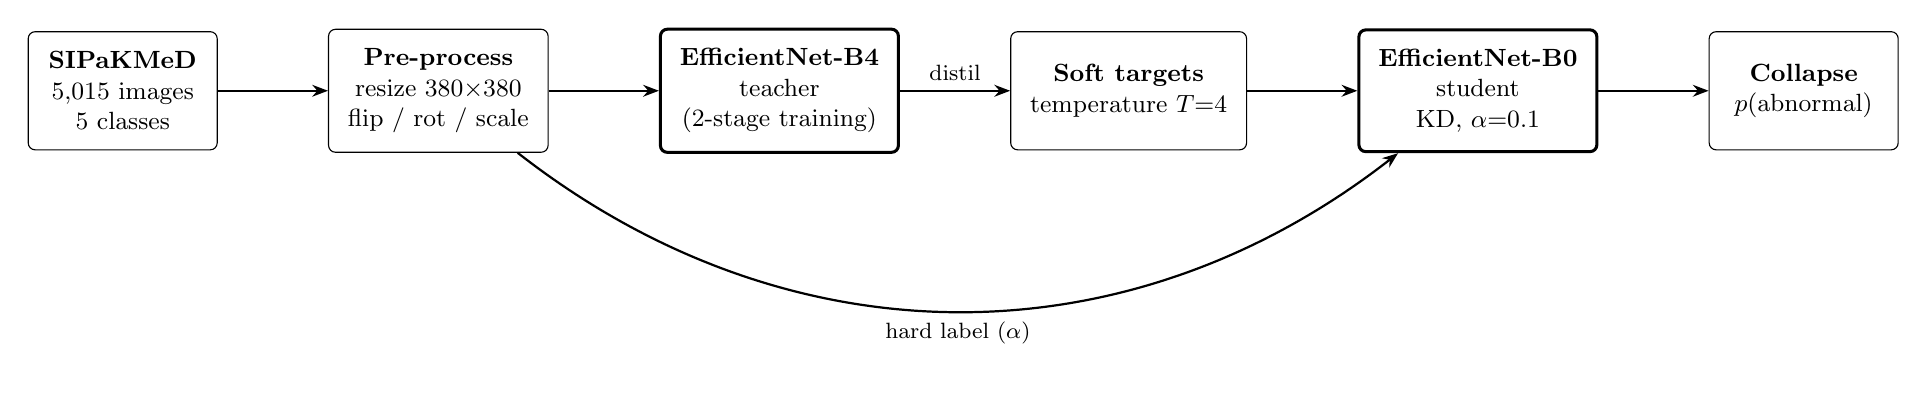
\begin{tikzpicture}[node distance=14mm, every node/.style={font=\small},
  pbox/.style={draw=black, fill=white, rounded corners=2.5pt, align=center, inner sep=7pt,
               minimum height=15mm, minimum width=24mm}, nbox/.style={pbox, line width=1.1pt}]
  \node[pbox] (d) {\textbf{SIPaKMeD}\\$5{,}015$ images\\$5$ classes};
  \node[pbox, right=of d] (aug) {\textbf{Pre-process}\\resize $380{\times}380$\\flip / rot / scale};
  \node[nbox, right=of aug] (t) {\textbf{EfficientNet-B4}\\teacher\\(2-stage training)};
  \node[pbox, right=of t] (soft) {\textbf{Soft targets}\\temperature $T{=}4$};
  \node[nbox, right=of soft] (s) {\textbf{EfficientNet-B0}\\student\\KD, $\alpha{=}0.1$};
  \node[pbox, right=of s] (out) {\textbf{Collapse}\\$p(\text{abnormal})$};
  \draw[fl](d)--(aug); \draw[fl](aug)--(t); \draw[fl](t)-- node[above, font=\footnotesize]{distil} (soft);
  \draw[fl](soft)--(s); \draw[fl](s)--(out);
  \draw[fl](aug) to[out=-38,in=-142] node[below, font=\footnotesize]{hard label ($\alpha$)} (s);
\end{tikzpicture}}
\caption{Cytology-expert training pipeline (left to right). Bold-bordered boxes are the trained networks: a
two-stage B4 teacher distils a B0 student ($T=4$, $\alpha=0.1$) whose five-class softmax is reduced to
$p(\text{abnormal})$.}
\Description{Left-to-right image-expert pipeline.}
\label{fig:imgpipe}
\end{figure*}

%% ---------------- TABULAR EXPERT METHOD ----------------
\subsection{HPV-risk expert}\label{sec:tabmethod}
\paragraph{Dataset and features.} Seven NHANES cycles (2003--2016) give $n=12{,}634$ women aged 18--59 with a
valid self-collected HPV swab, merged on the respondent identifier across the demographic, sexual-behaviour,
reproductive, smoking, and immunisation questionnaires. The label is high-risk HPV positivity (any of 14
oncogenic genotypes on the Roche Linear Array), present in $24.6\%$ of the cohort. The features are $30$
questionnaire items plus engineered exposure ratios (e.g.\ lifetime partners per sexually-active year).

\paragraph{Model.} Missing values are median-imputed; class imbalance is handled by class
weights rather than synthetic oversampling~\cite{chawla2002}, so every model is trained on the real $12{,}634$
records; the data are modelled with a RandomForest ensemble ($600$ trees, balanced class weights) and
probabilities are isotonic-calibrated. Figure~\ref{fig:tabpipe} summarises the pipeline; model selection is
detailed in \S\ref{sec:setup}.

\begin{figure*}[t]\centering
\resizebox{0.98\textwidth}{!}{%
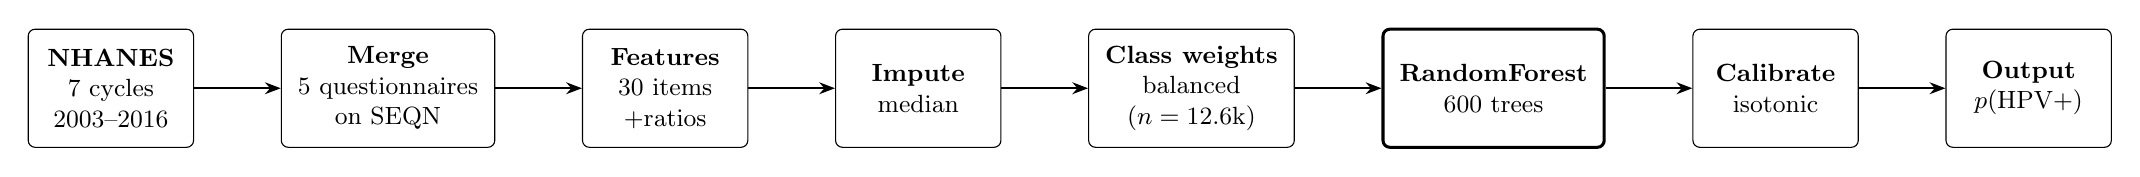
\begin{tikzpicture}[node distance=11mm, every node/.style={font=\small},
  pbox/.style={draw=black, fill=white, rounded corners=2.5pt, align=center, inner sep=6pt,
               minimum height=15mm, minimum width=21mm}, nbox/.style={pbox, line width=1.1pt}]
  \node[pbox] (n) {\textbf{NHANES}\\7 cycles\\2003--2016};
  \node[pbox, right=of n] (m) {\textbf{Merge}\\5 questionnaires\\on SEQN};
  \node[pbox, right=of m] (fe) {\textbf{Features}\\30 items\\+ratios};
  \node[pbox, right=of fe] (c) {\textbf{Impute}\\median};
  \node[pbox, right=of c] (sm) {\textbf{Class weights}\\balanced\\($n=12.6$k)};
  \node[nbox, right=of sm] (rf) {\textbf{RandomForest}\\600 trees};
  \node[pbox, right=of rf] (cal) {\textbf{Calibrate}\\isotonic};
  \node[pbox, right=of cal] (o) {\textbf{Output}\\$p(\text{HPV{+}})$};
  \draw[fl](n)--(m); \draw[fl](m)--(fe); \draw[fl](fe)--(c); \draw[fl](c)--(sm);
  \draw[fl](sm)--(rf); \draw[fl](rf)--(cal); \draw[fl](cal)--(o);
\end{tikzpicture}}
\caption{HPV-risk-expert training pipeline (left to right). Seven NHANES cycles are merged into a $30$-feature
table, imputed, class-weighted to offset imbalance, modelled with RandomForest, and isotonic-calibrated to
$p(\text{HPV+})$. The bold-bordered box is the trained model.}
\Description{Left-to-right tabular-expert pipeline.}
\label{fig:tabpipe}
\end{figure*}

%% ---------------- FUSION METHOD ----------------
\subsection{Decision-level fusion}\label{sec:fusmethod}
\paragraph{Step 1 --- CO-PRIOR.} Each expert is calibrated to its own base rate, so before pooling we strip
that prior and install the deployment prevalence $\tau$:
\begin{equation}\label{eq:coprior}
\operatorname{logit}\hat p \;=\; \operatorname{logit} p \;-\; \operatorname{logit}\pi \;+\; \operatorname{logit}\tau .
\end{equation}
\emph{Reading Eq.~\eqref{eq:coprior}:} $p$ is a raw posterior, $\pi$ its training prevalence, $\tau$ the
deployment prevalence; subtracting $\operatorname{logit}\pi$ removes the trained-in base rate and adding
$\operatorname{logit}\tau$ installs the deployment one. The single-classifier form of this adjustment is due
to Saerens et al.~\cite{saerens2002}; the contribution here is applying it \emph{independently to each
heterogeneous expert before} decision-level pooling, so that two models with different priors become
comparable.

\paragraph{Step 2 --- combine.} We pool the re-anchored posteriors with the Kittler sum
rule~\cite{kittler1998}, $p_{\mathrm{sum}}=\tfrac12(\hat p_{\mathrm{img}}+\hat p_{\mathrm{tab}})$.

\paragraph{Step 3 --- asymmetric cascade (engineering safety heuristic).} As a design choice---not a
clinically validated rule---the combiner does not let a low questionnaire score reduce a high cytology score:
$p_{\mathrm{fused}}=\max(p_{\mathrm{sum}},\hat p_{\mathrm{img}})$ when $\hat p_{\mathrm{img}}\ge\theta$, else
$p_{\mathrm{sum}}$. This prevents the questionnaire from suppressing a positive cytological signal above the
threshold $\theta$.

\paragraph{Step 4 --- abstain.} Each expert carries split-conformal thresholds~\cite{angelopoulos2023}
calibrated on its own data; ambiguous or lone-weak cases return \textsc{defer}, substantial disagreement returns
\textsc{flag}, otherwise \textsc{release}.

%% =====================================================================
\section{Experimental setup}\label{sec:setup}
\paragraph{Data splits.} The cytology expert uses a stratified $80/20$ train/validation split of SIPaKMeD
(seed $42$); all reported cytology numbers are on this \emph{validation} split (there is no separate held-out
test set---see \S\ref{sec:limits}). The HPV-risk expert is evaluated by stratified $5$-fold cross-validation
on NHANES. Cross-dataset transfer uses Herlev, APACC, and HiCervix as external image sets.
\paragraph{Metrics.} We report accuracy, balanced accuracy, macro-AUROC, F1, precision, recall, and, for
probability quality, expected calibration error (ECE) with reliability diagrams. Discrimination (AUROC) is
threshold-free; the operating-point metrics use a $0.5$ threshold unless stated.
\paragraph{Model selection.} For the HPV-risk expert we compared ExtraTrees, RandomForest, XGBoost,
LightGBM~\cite{ke2017lightgbm}, and $k$-NN under the same $5$-fold protocol; gradient-boosted families were
tuned with Optuna~\cite{akiba2019optuna} (tree-structured Parzen sampler, objective = CV AUROC). RandomForest
($600$ trees, balanced class weights) gave the highest CV AUROC and is used throughout; its probabilities are
isotonic-calibrated.
\paragraph{Fusion evaluation.} Because no patient has both modalities, the fusion is analysed per expert
(calibration, conformal coverage) and on a deployment cohort constructed from the experts' real per-class
score distributions to study prevalence re-anchoring and combiner behaviour.

%% =====================================================================
\section{Results}
Results are grouped by component: the cytology expert (\S\ref{sec:imgres}), the HPV-risk expert
(\S\ref{sec:tabres}), and the fused system (\S\ref{sec:fusres}).

%% ================= IMAGE EXPERT RESULTS =================
\subsection{Cytology expert}\label{sec:imgres}
\paragraph{Dataset.} The five morphology classes are near-balanced (imbalance ratio $1.19$;
Figure~\ref{fig:eda_bal}), so no class dominates training; Figure~\ref{fig:eda_cells} shows one cell per class.

\begin{figure}[tb]\centering
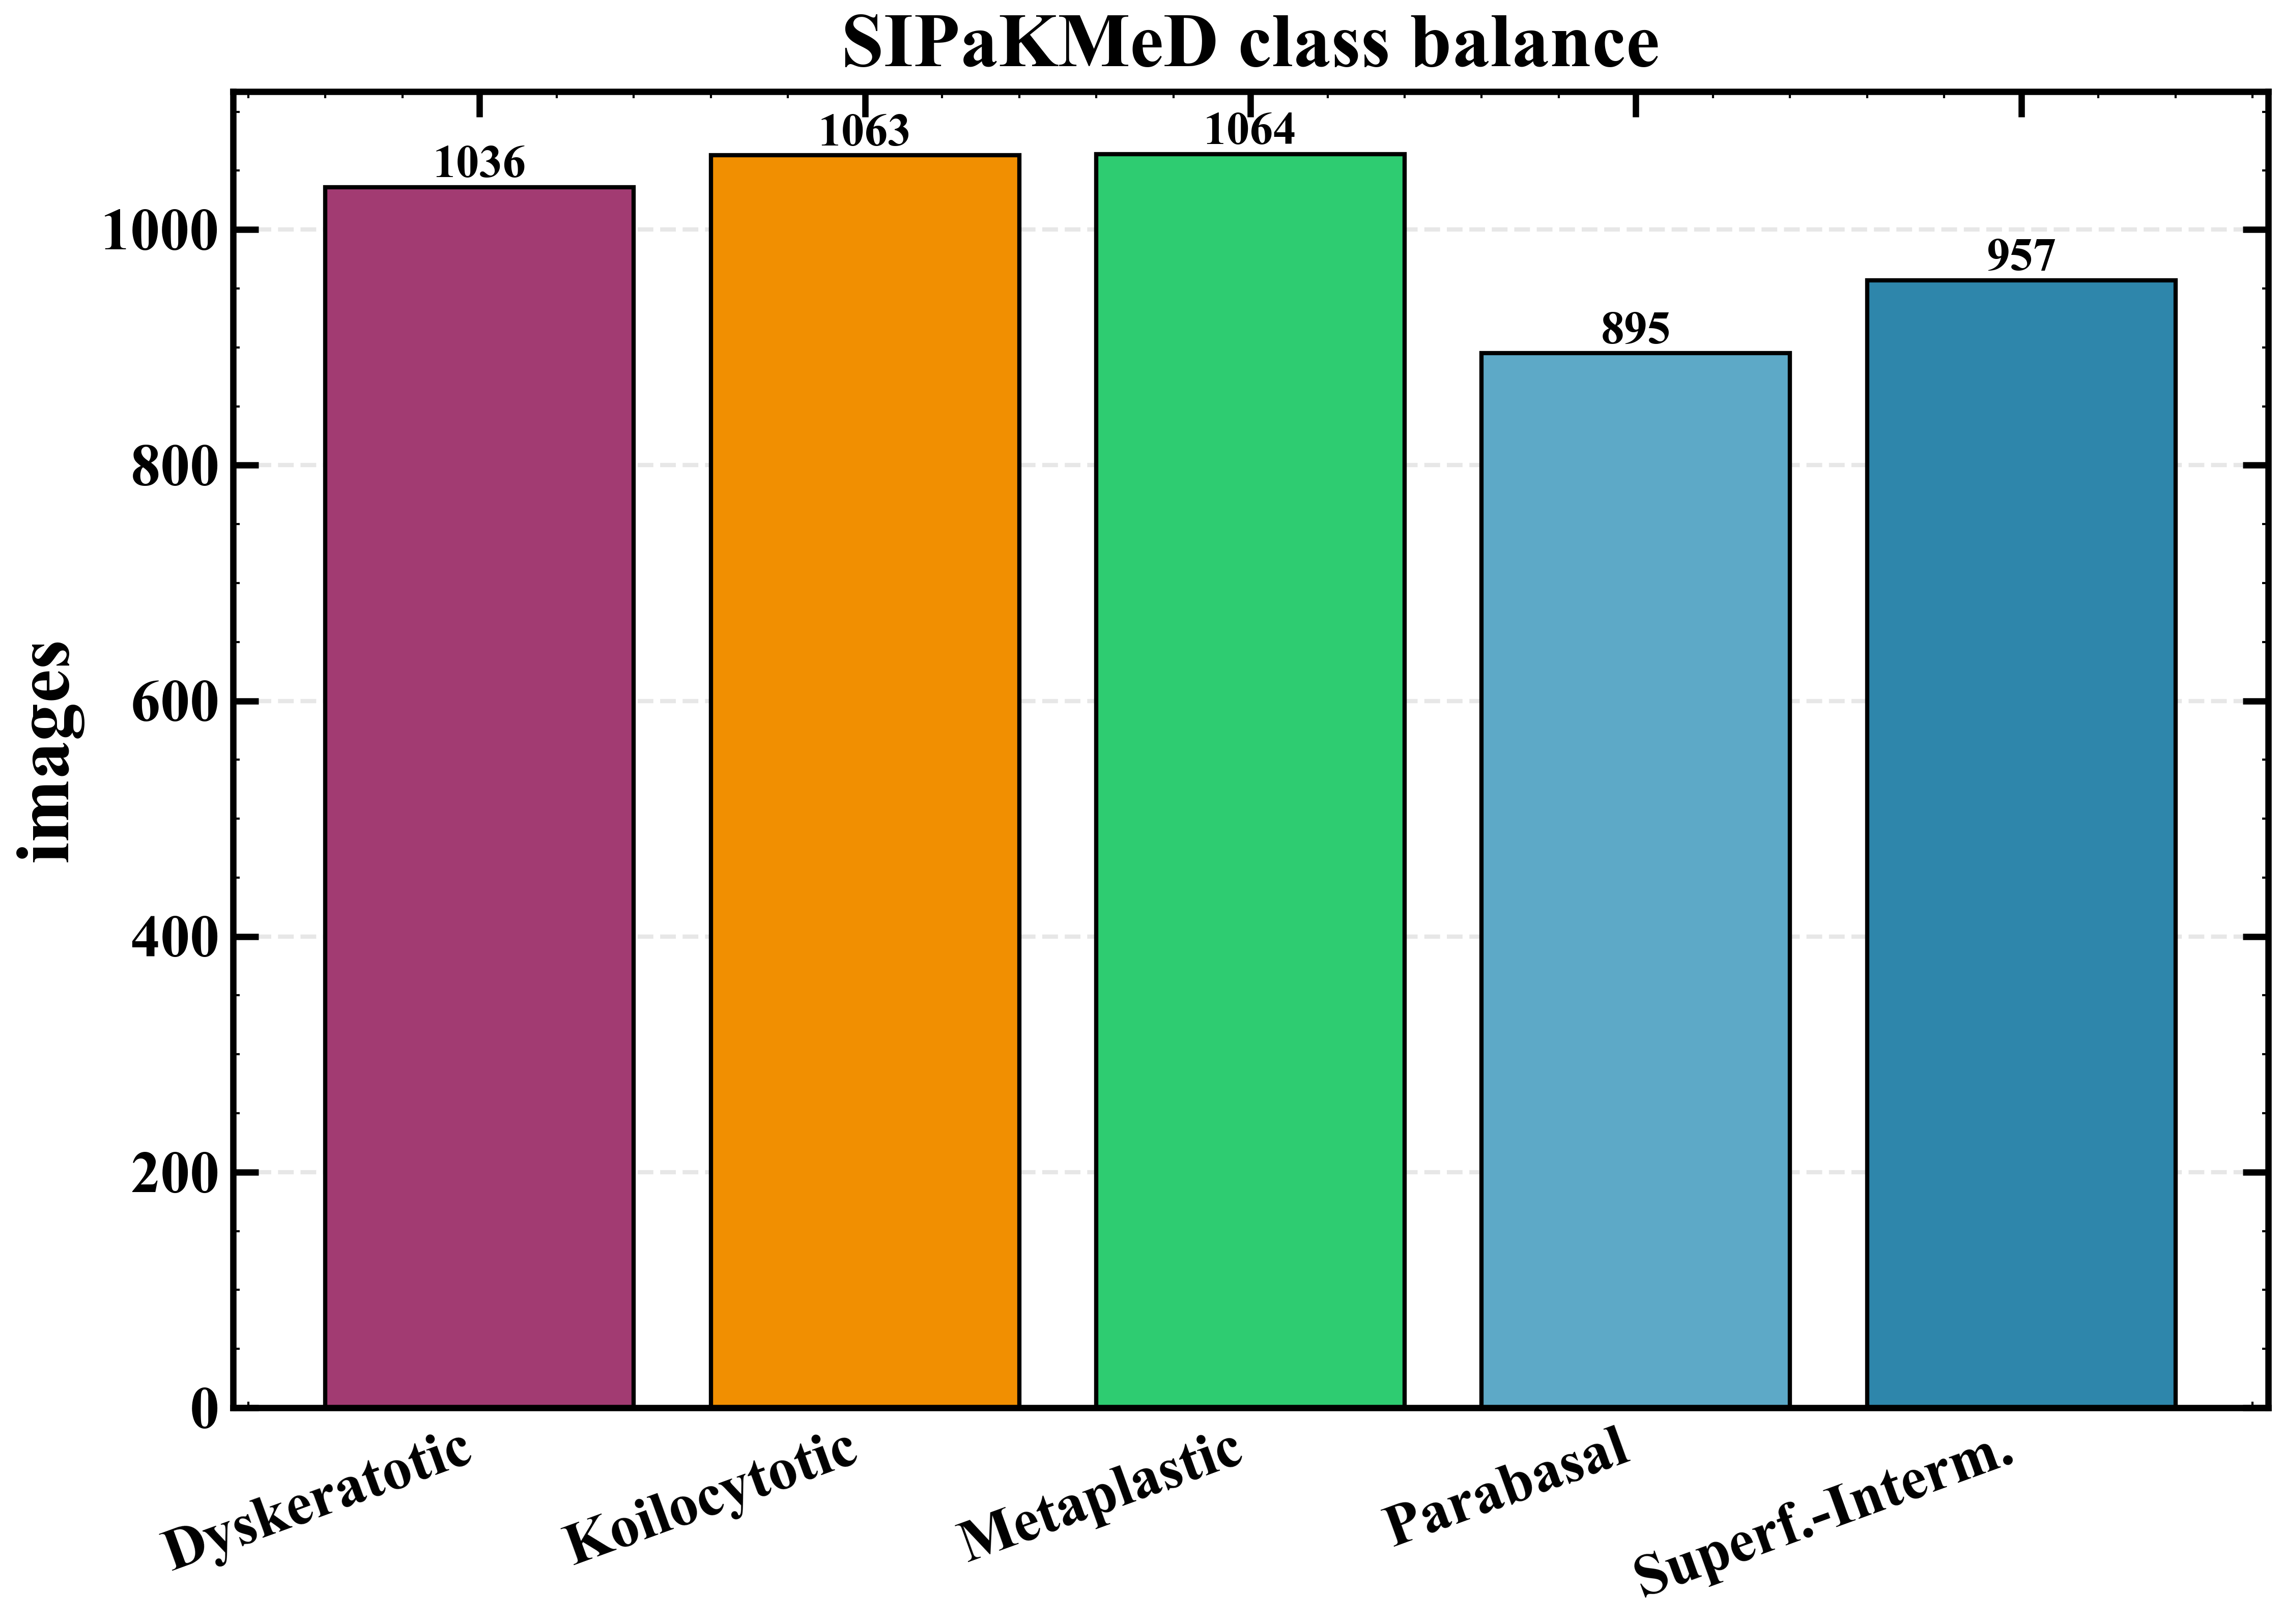
\includegraphics[width=0.86\columnwidth]{figures/eda_class_balance.png}
\caption{SIPaKMeD images per morphology class (imbalance ratio $1.19$).}
\Description{Bar chart of images per class.}
\label{fig:eda_bal}
\end{figure}

\begin{figure}[tb]\centering
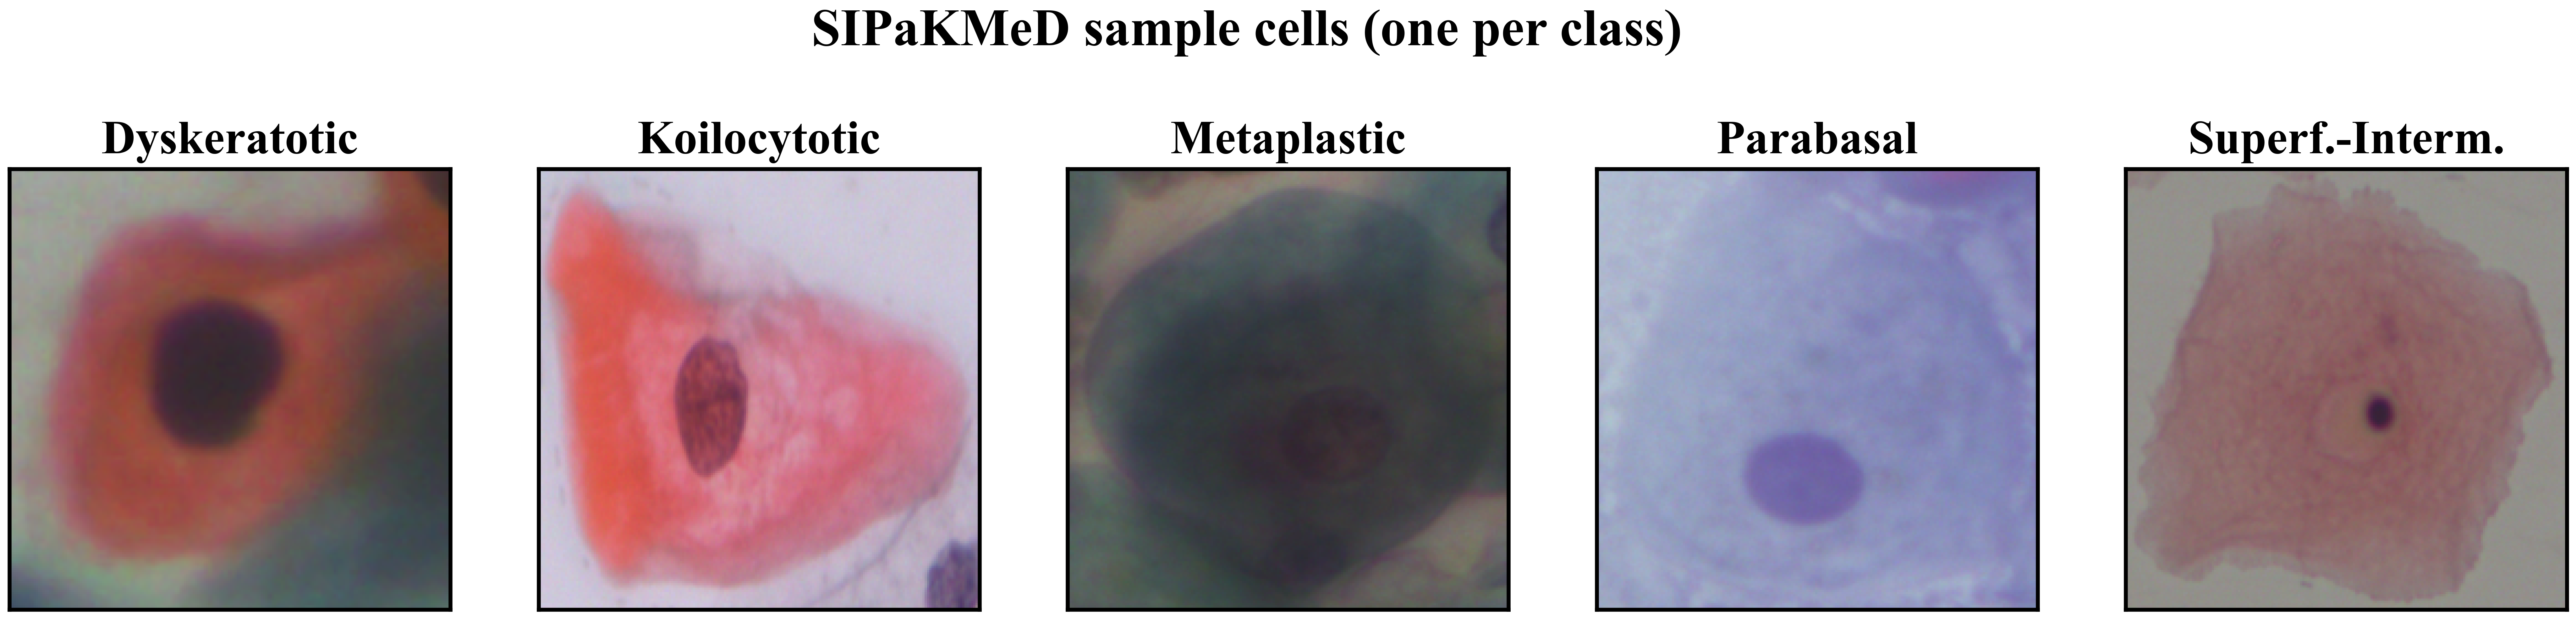
\includegraphics[width=0.98\columnwidth]{figures/eda_sample_cells.png}
\caption{One representative cell per SIPaKMeD class.}
\Description{Panel of five sample cell images.}
\label{fig:eda_cells}
\end{figure}

\paragraph{Classification performance.} On the validation split the distilled student attains $0.966$
accuracy, $0.968$ balanced accuracy, and $0.998$ macro-AUROC (Table~\ref{tab:img}), exceeding the larger
teacher despite having roughly a quarter of the parameters ($\sim4$M vs $\sim17.5$M). Balanced accuracy equal
to accuracy indicates the model is not exploiting a majority class. Training and validation curves
(Figure~\ref{fig:train}) converge without a growing train/validation gap. Because these are validation-split
numbers, they should be read as in-distribution performance, not as an independent test estimate.

\begin{table}[tb]\centering\footnotesize\setlength{\tabcolsep}{5pt}
\caption{Cytology expert: five-class validation-split performance and external transfer (student).}
\label{tab:img}
\begin{tabular}{@{}lcccc@{}}
\toprule
\textbf{Setting} & \textbf{Acc} & \textbf{Bal.\ acc} & \textbf{AUROC} & \textbf{ECE}\\
\midrule
Teacher B4 (SIPaKMeD val) & 0.943 & 0.946 & 0.995 & 0.013\\
\textbf{Student B0 (SIPaKMeD val)} & \textbf{0.966} & \textbf{0.968} & \textbf{0.998} & 0.016\\
Student, Herlev~\cite{jantzen2005} & --- & 0.651 & 0.728 & ---\\
Student, APACC & --- & 0.535 & --- & ---\\
Student, HiCervix & --- & 0.562 & --- & ---\\
\bottomrule
\end{tabular}
\end{table}

\begin{figure}[tb]\centering
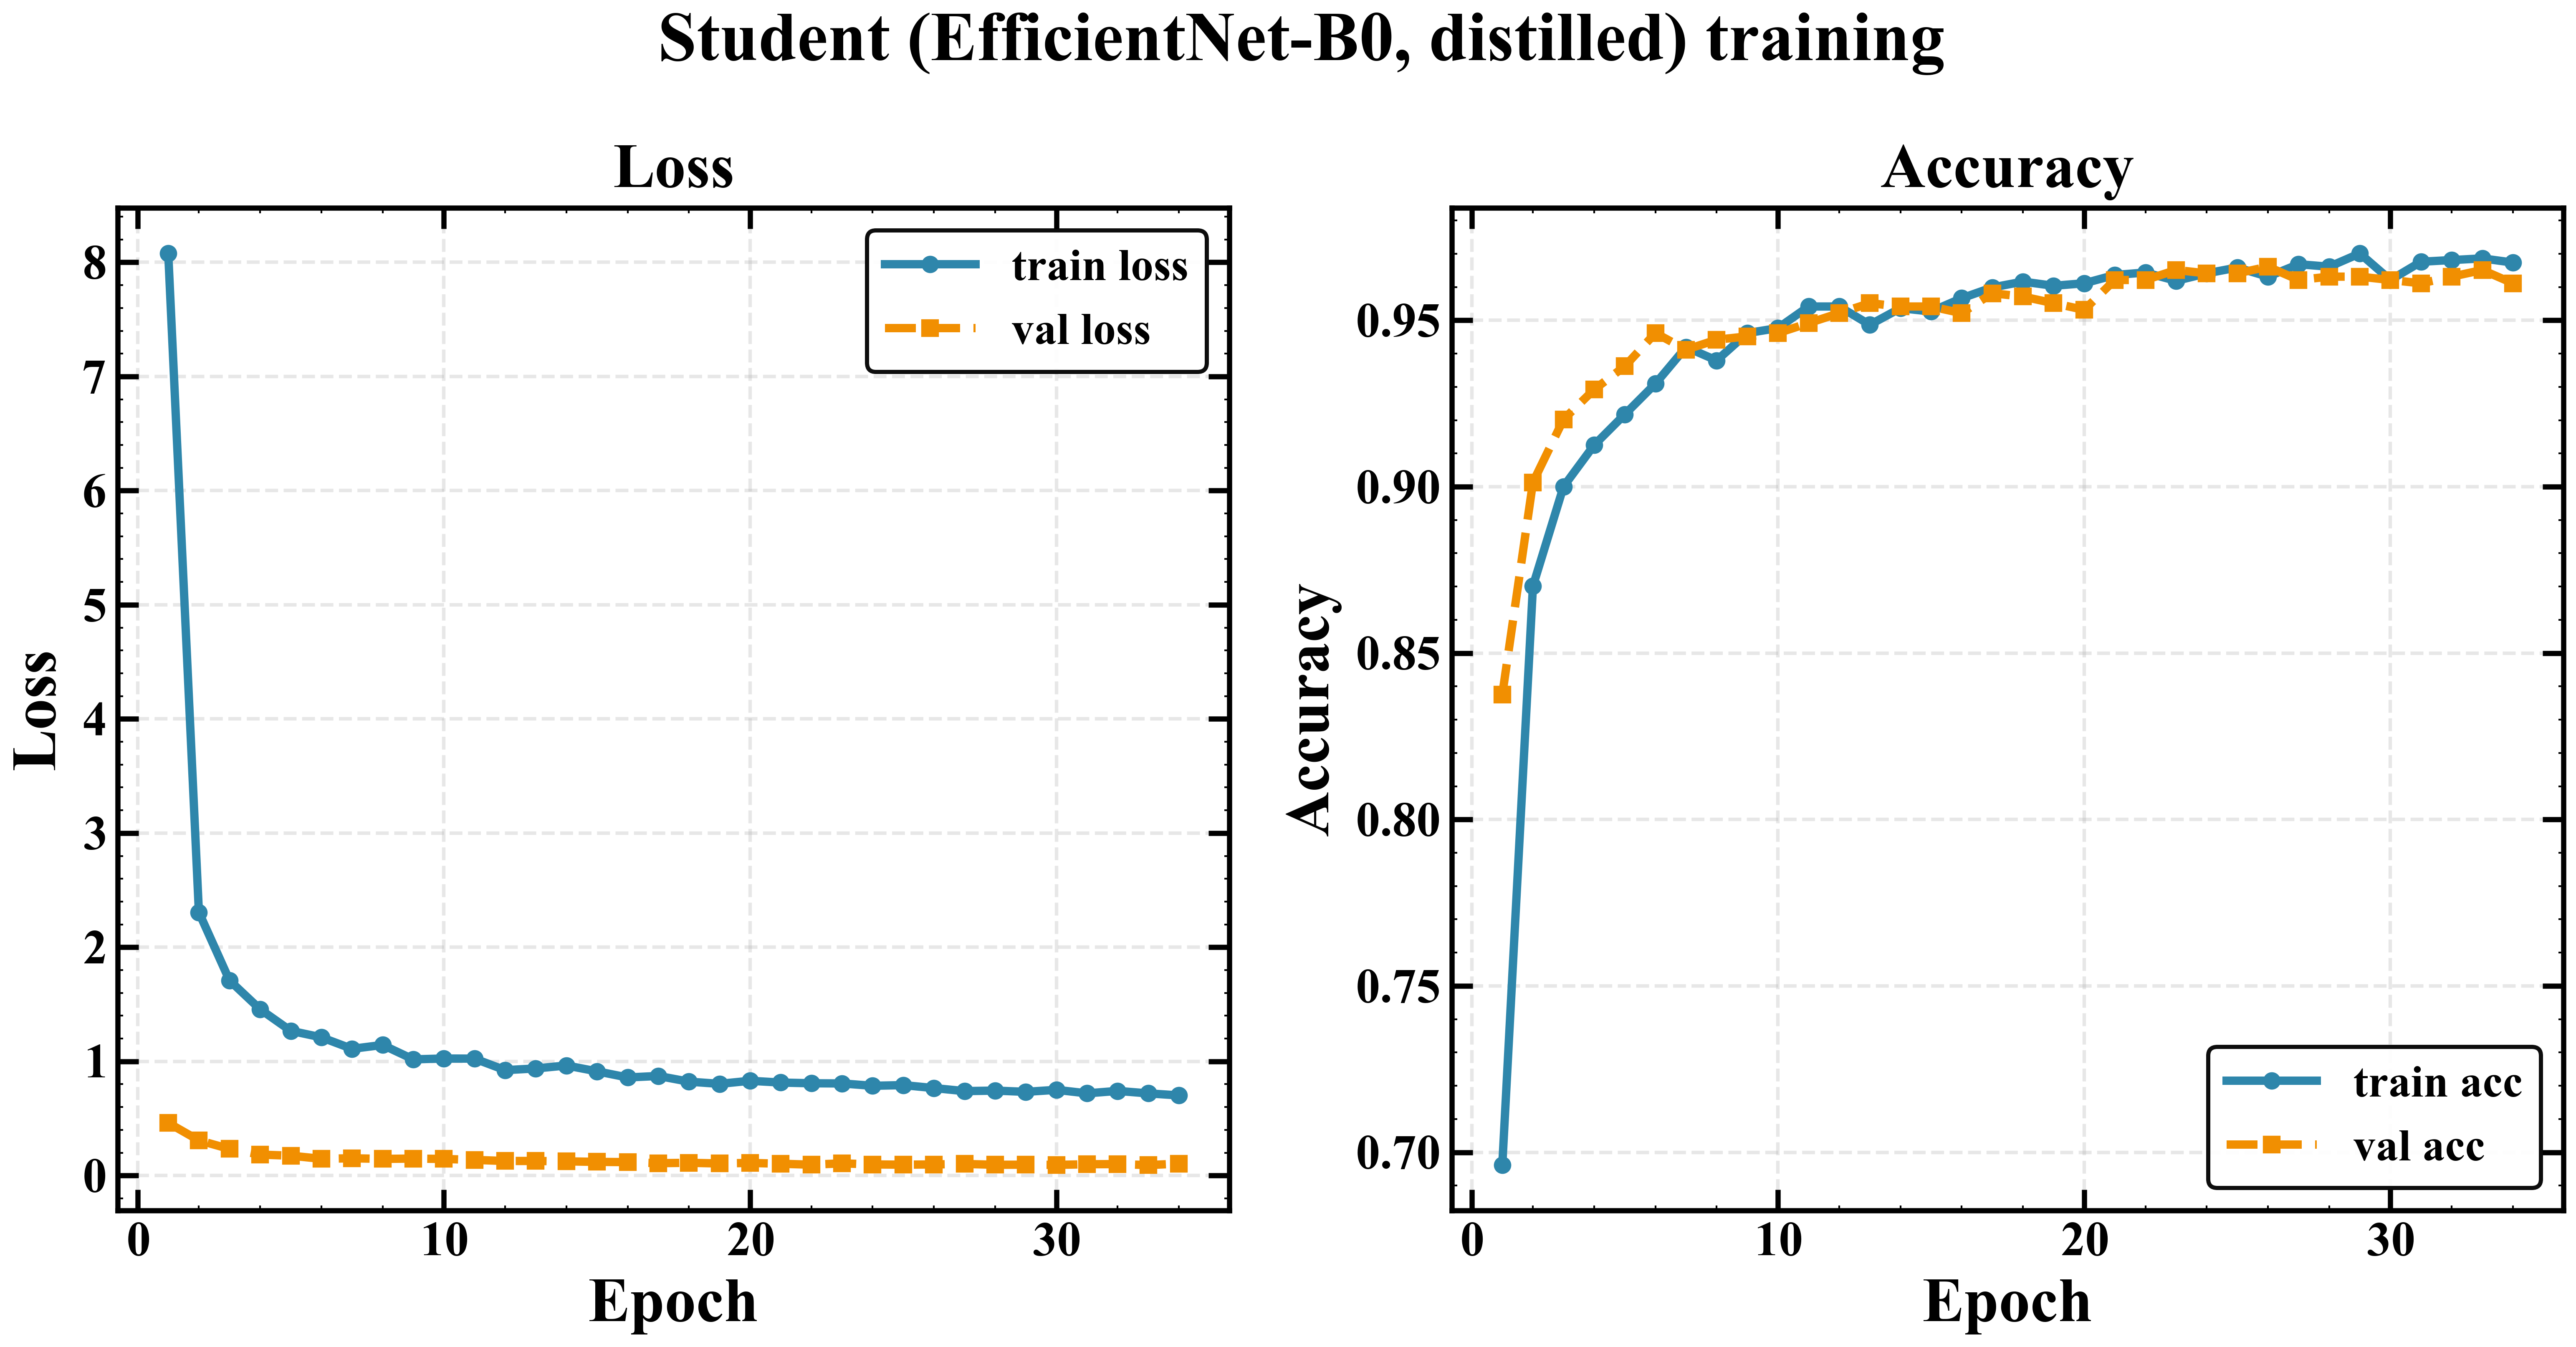
\includegraphics[width=\columnwidth]{figures/train_curves.png}
\caption{Student training/validation loss and accuracy across distillation epochs.}
\Description{Loss and accuracy curves.}
\label{fig:train}
\end{figure}

\paragraph{Errors, discrimination, calibration.} The confusion matrix (Figure~\ref{fig:cm}) is diagonal, with
residual confusions between morphologically adjacent classes. The per-class ROC curves and the reliability
diagram (Figure~\ref{fig:rocrel}) give ECE $=0.016$, indicating close agreement between predicted
probabilities and empirical frequencies on the validation split.

\begin{figure}[tb]\centering
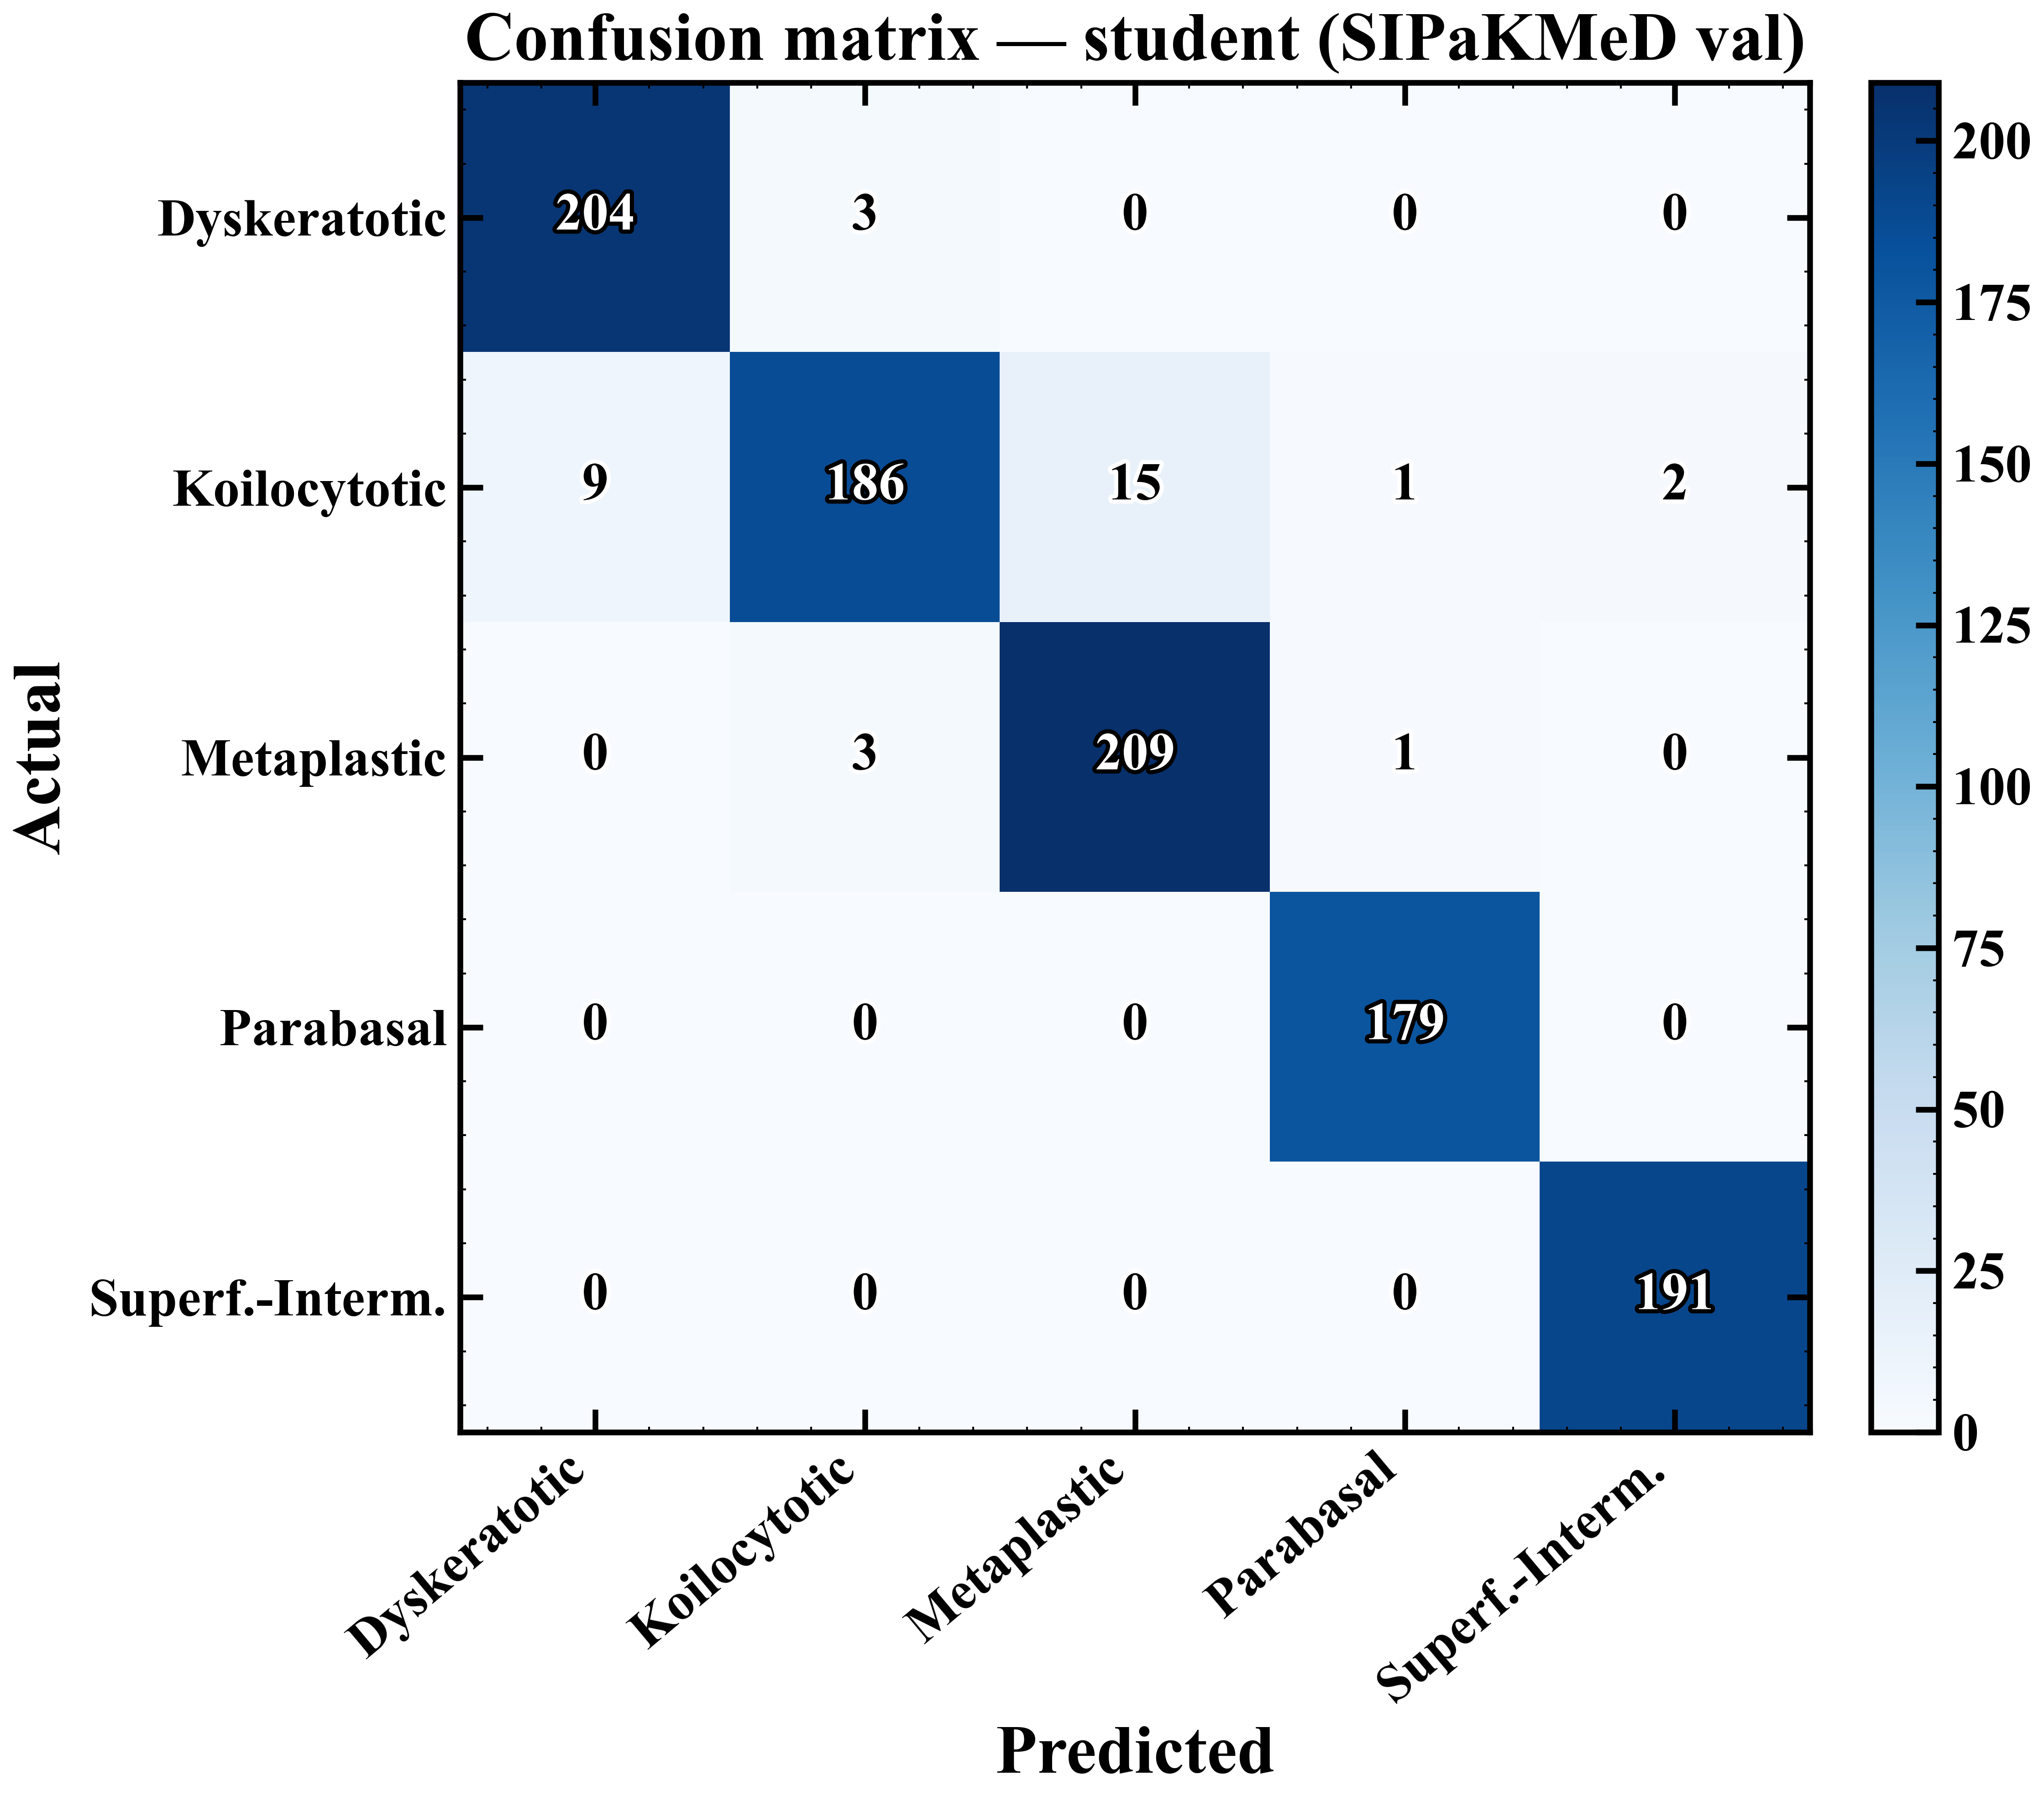
\includegraphics[width=0.8\columnwidth]{figures/cm_student.png}
\caption{Student five-class confusion matrix (SIPaKMeD validation split).}
\Description{Five-by-five confusion matrix.}
\label{fig:cm}
\end{figure}

\begin{figure}[tb]\centering
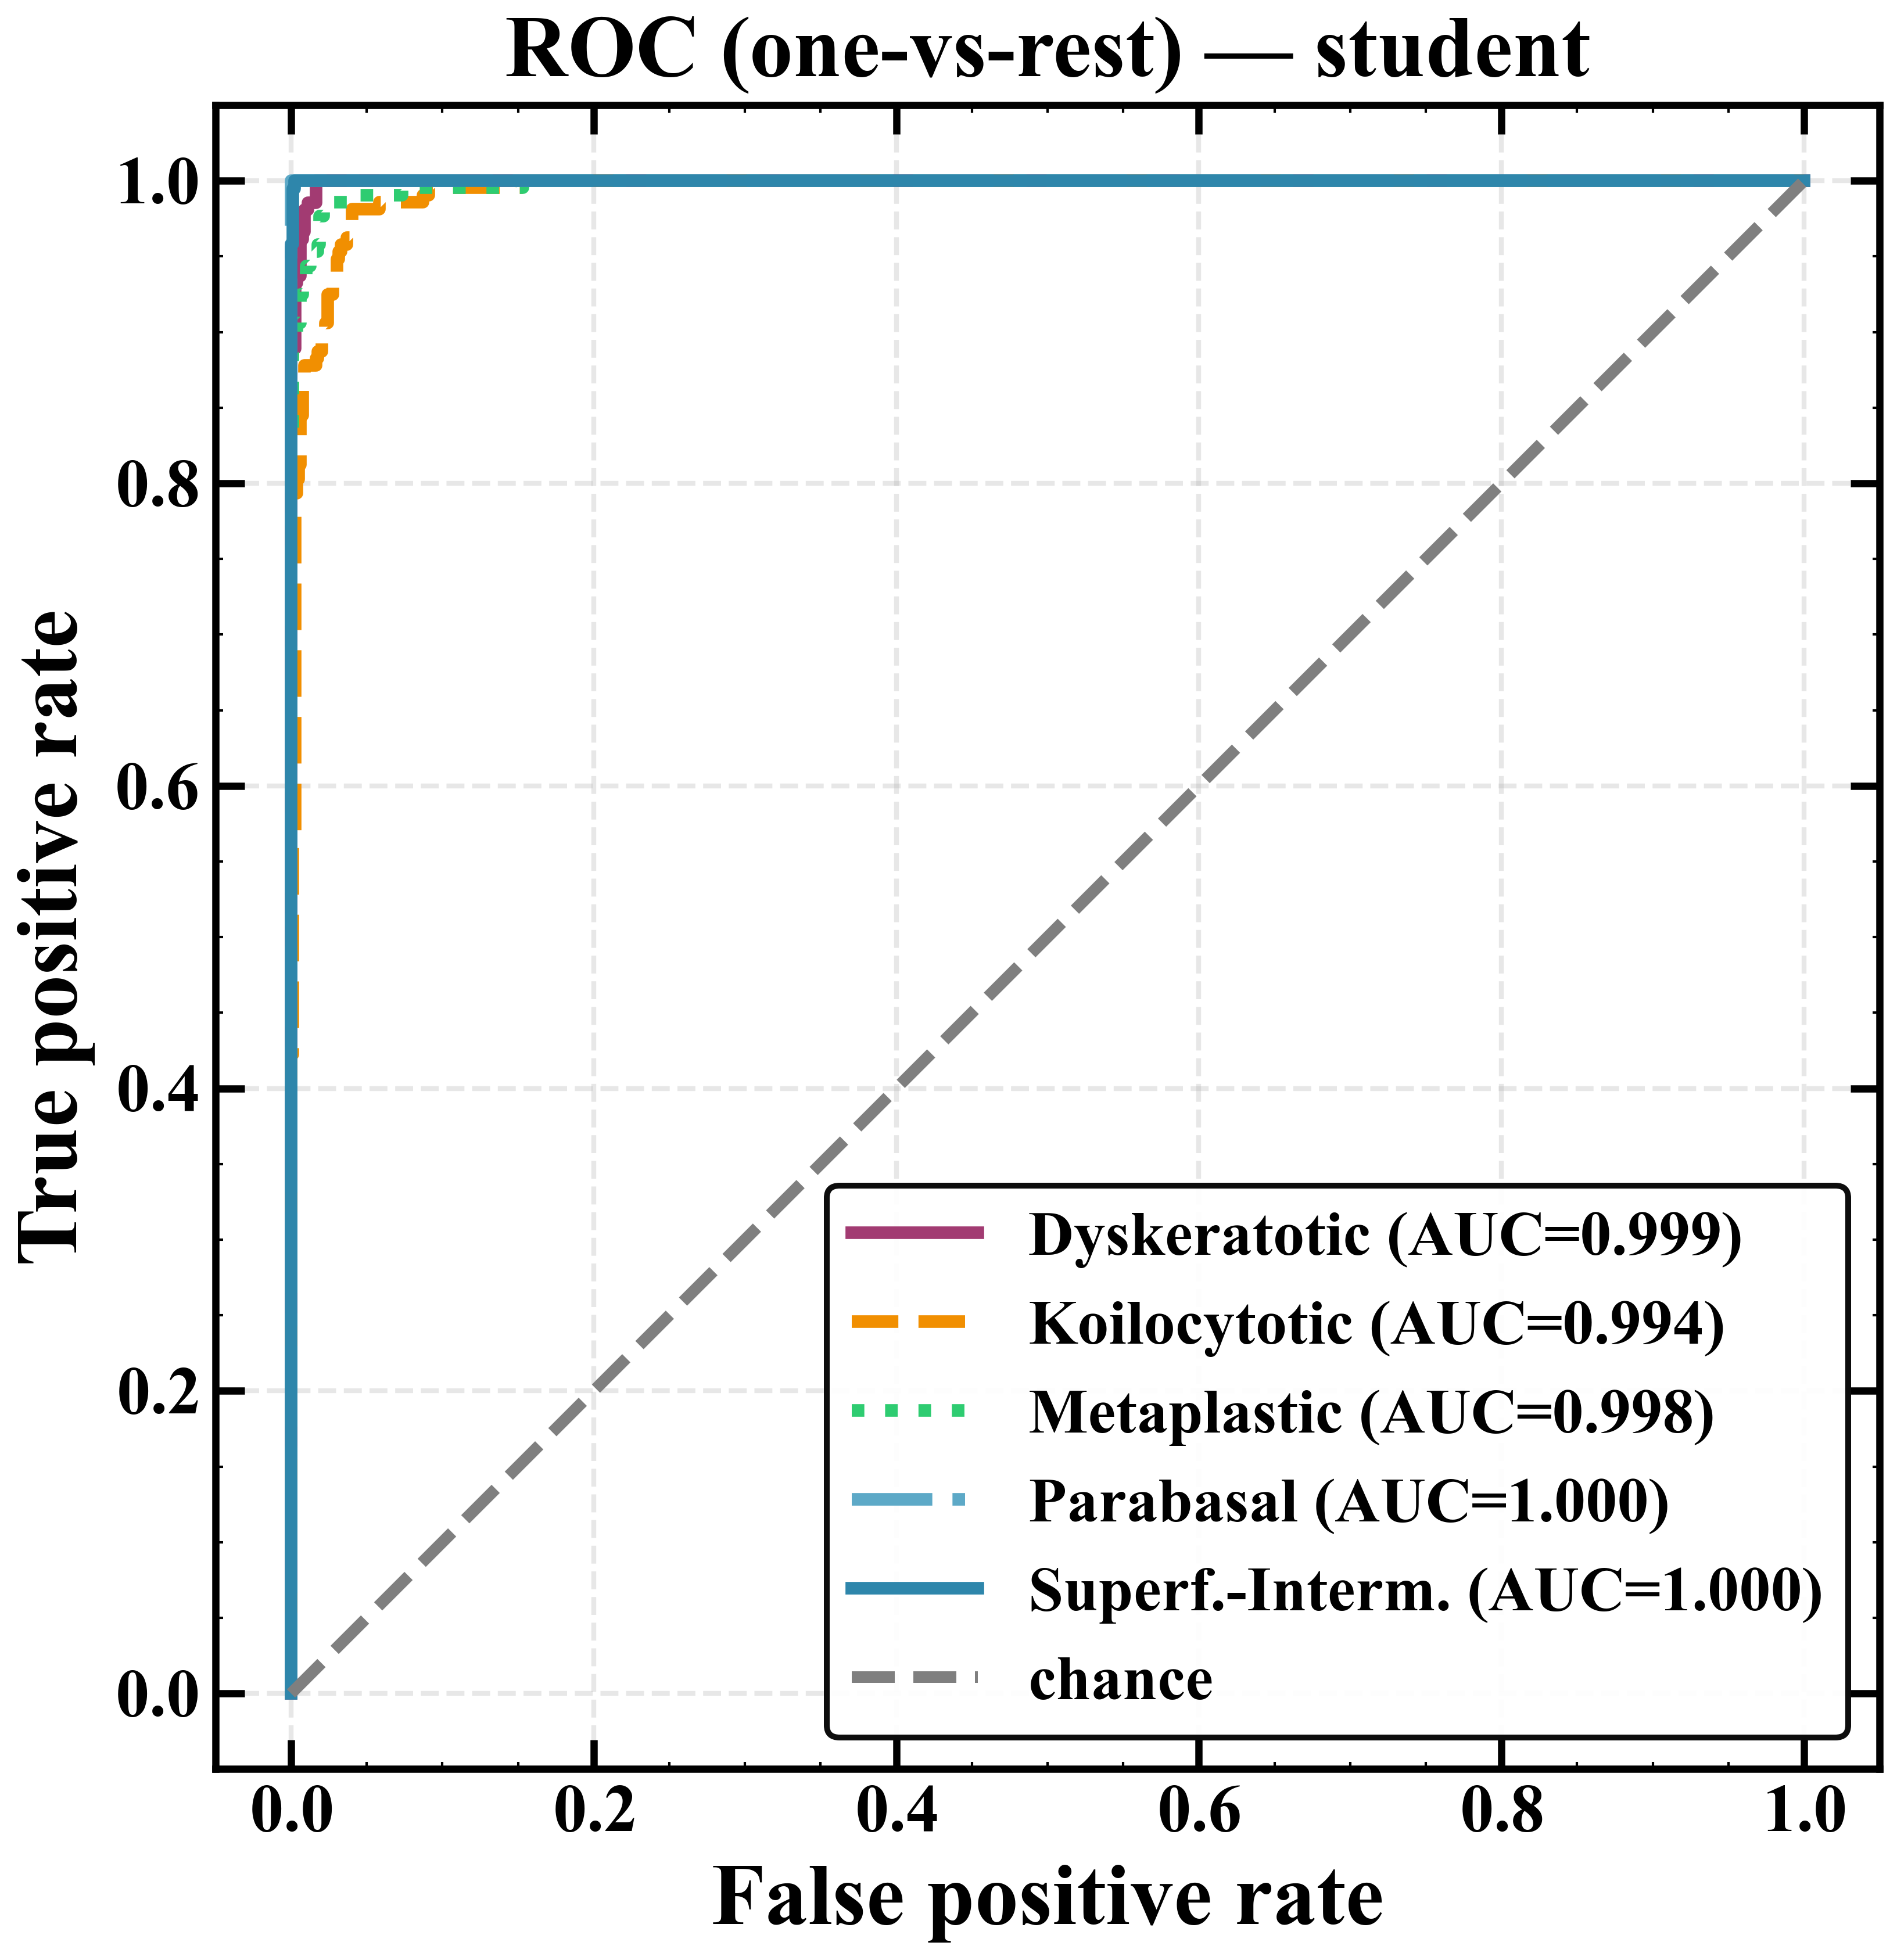
\includegraphics[width=0.49\columnwidth]{figures/roc_student.png}\hfill
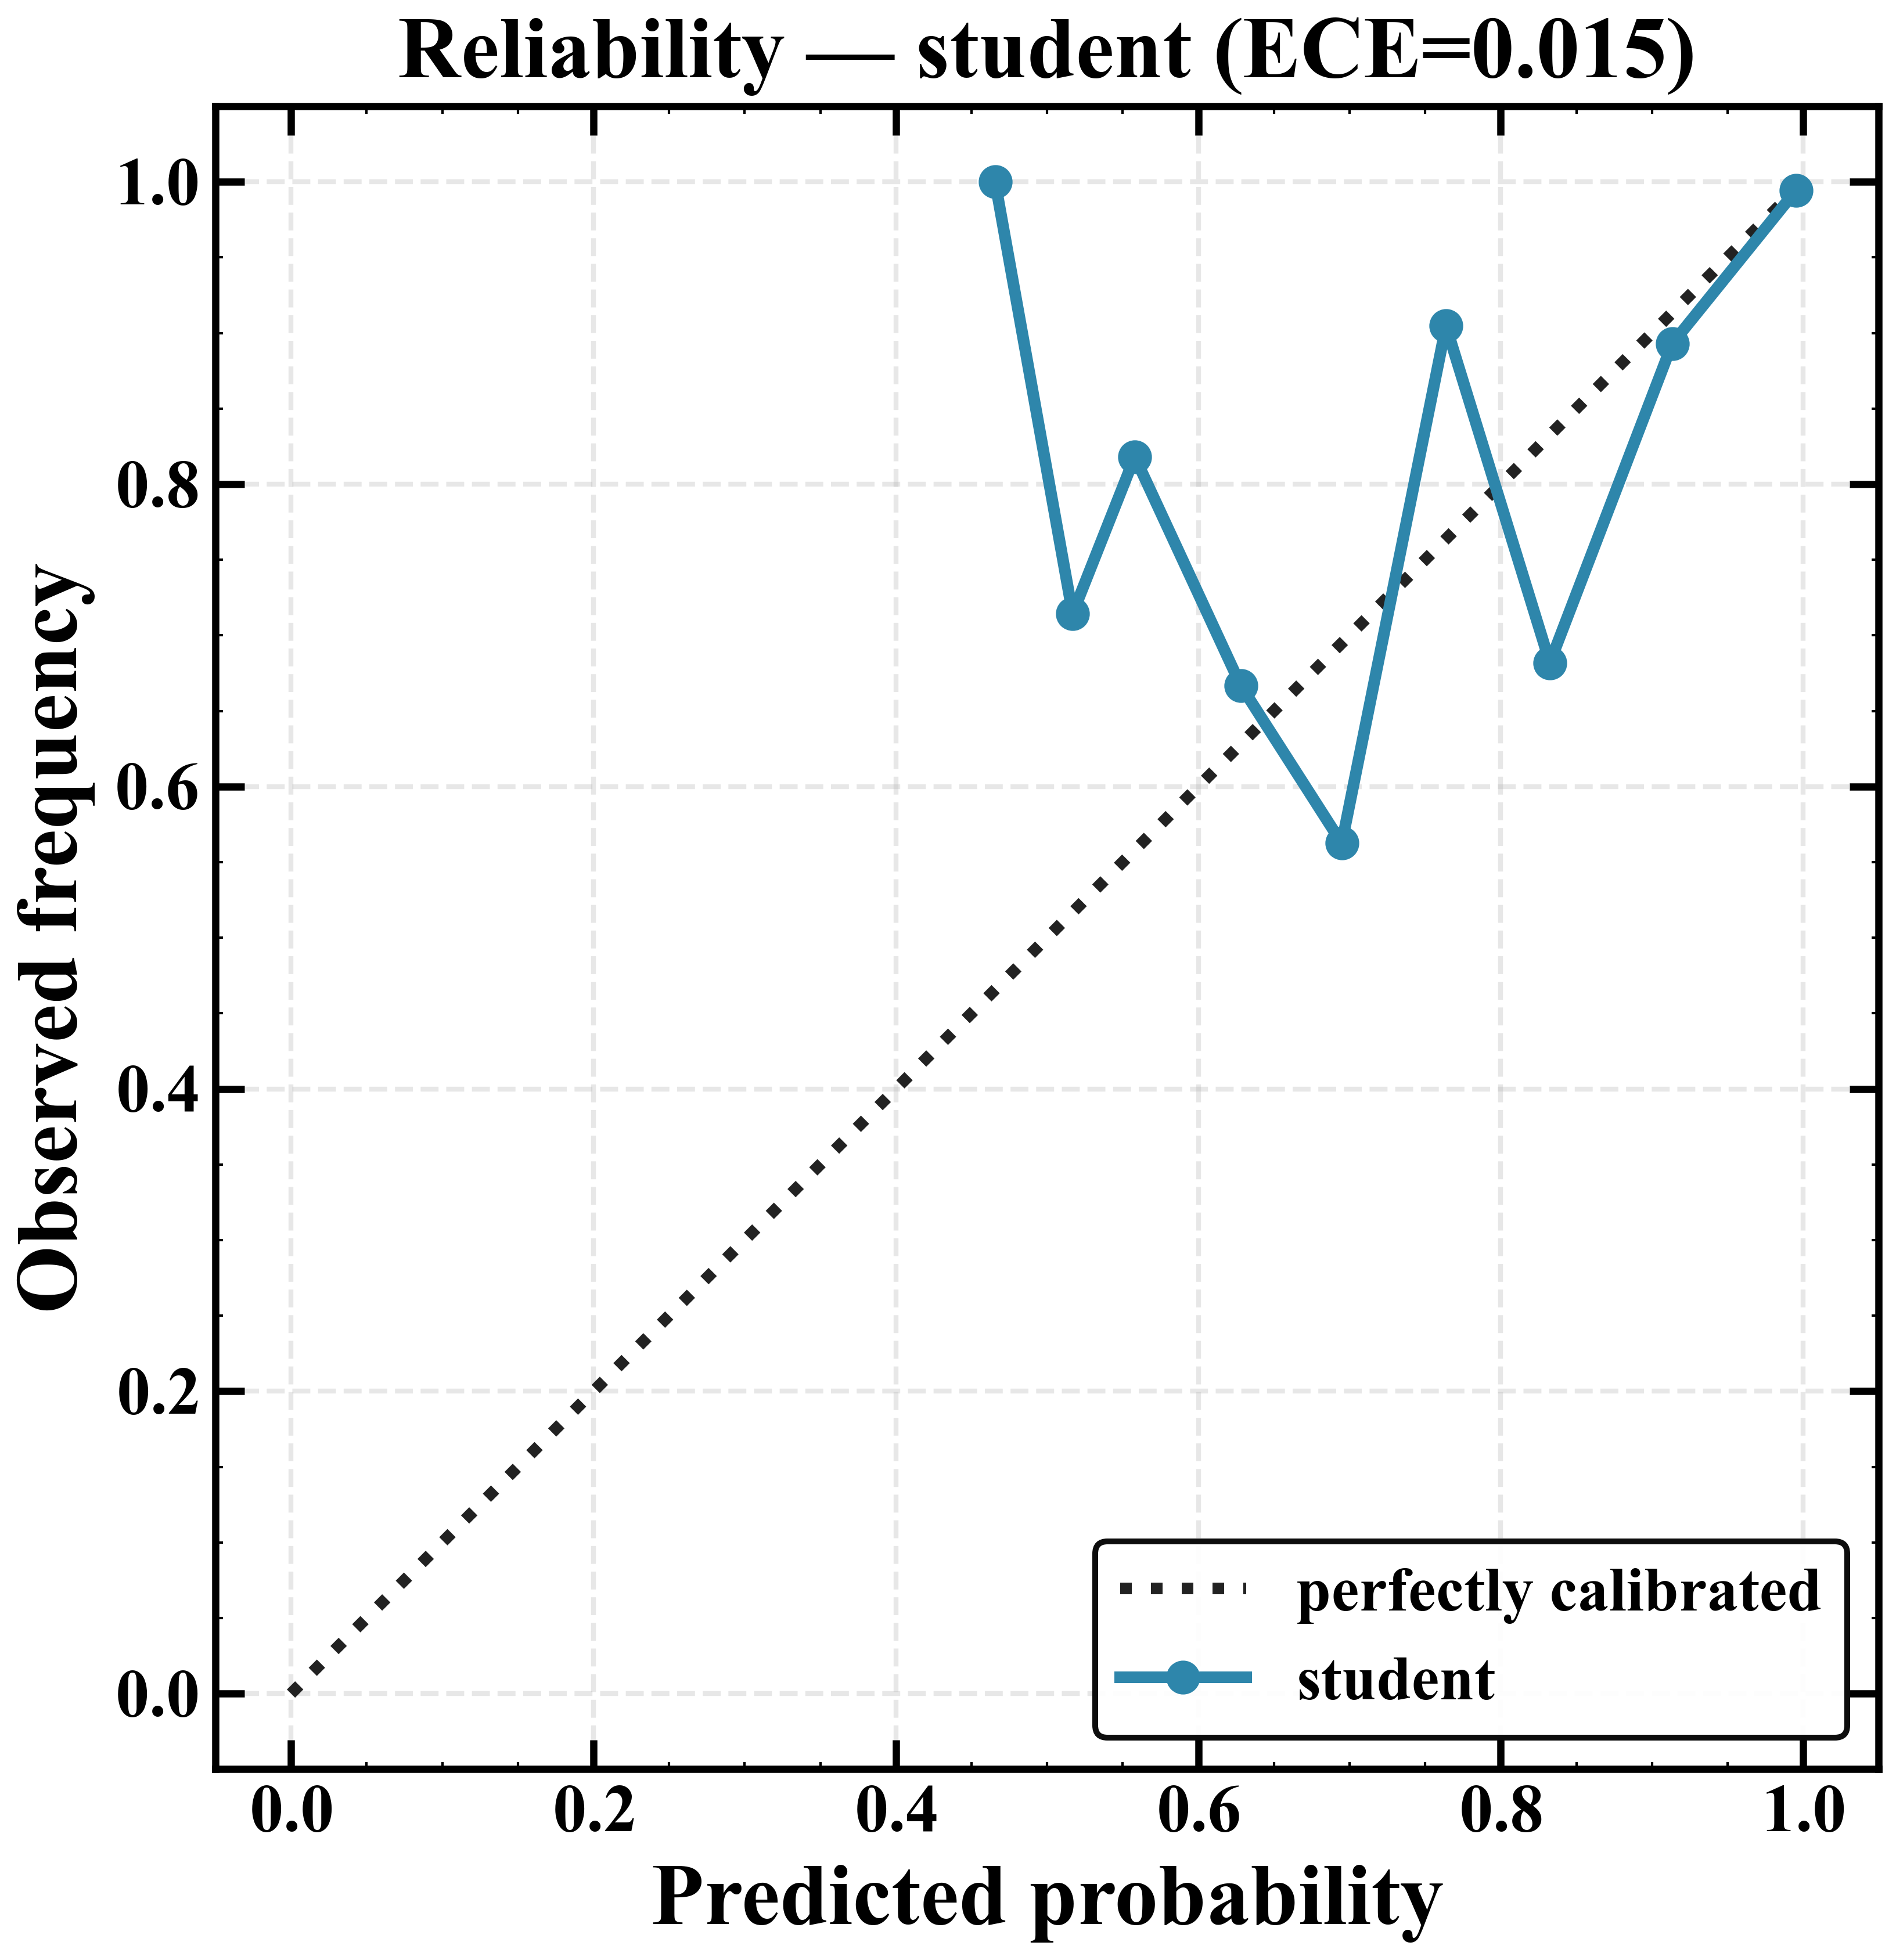
\includegraphics[width=0.49\columnwidth]{figures/reliability_student.png}
\caption{Student ROC curves (left) and reliability diagram (right; ECE $=0.016$).}
\Description{ROC curves and reliability diagram.}
\label{fig:rocrel}
\end{figure}

\paragraph{Attribution.} Grad-CAM~\cite{selvaraju2017} for the abnormal-class logit indicates that
attribution concentrates on nuclear and perinuclear regions (Figure~\ref{fig:gradcam}); this localises the
gradient signal to morphologically relevant regions but does not by itself establish that the model uses the
underlying biological mechanism.

\begin{figure}[tb]\centering
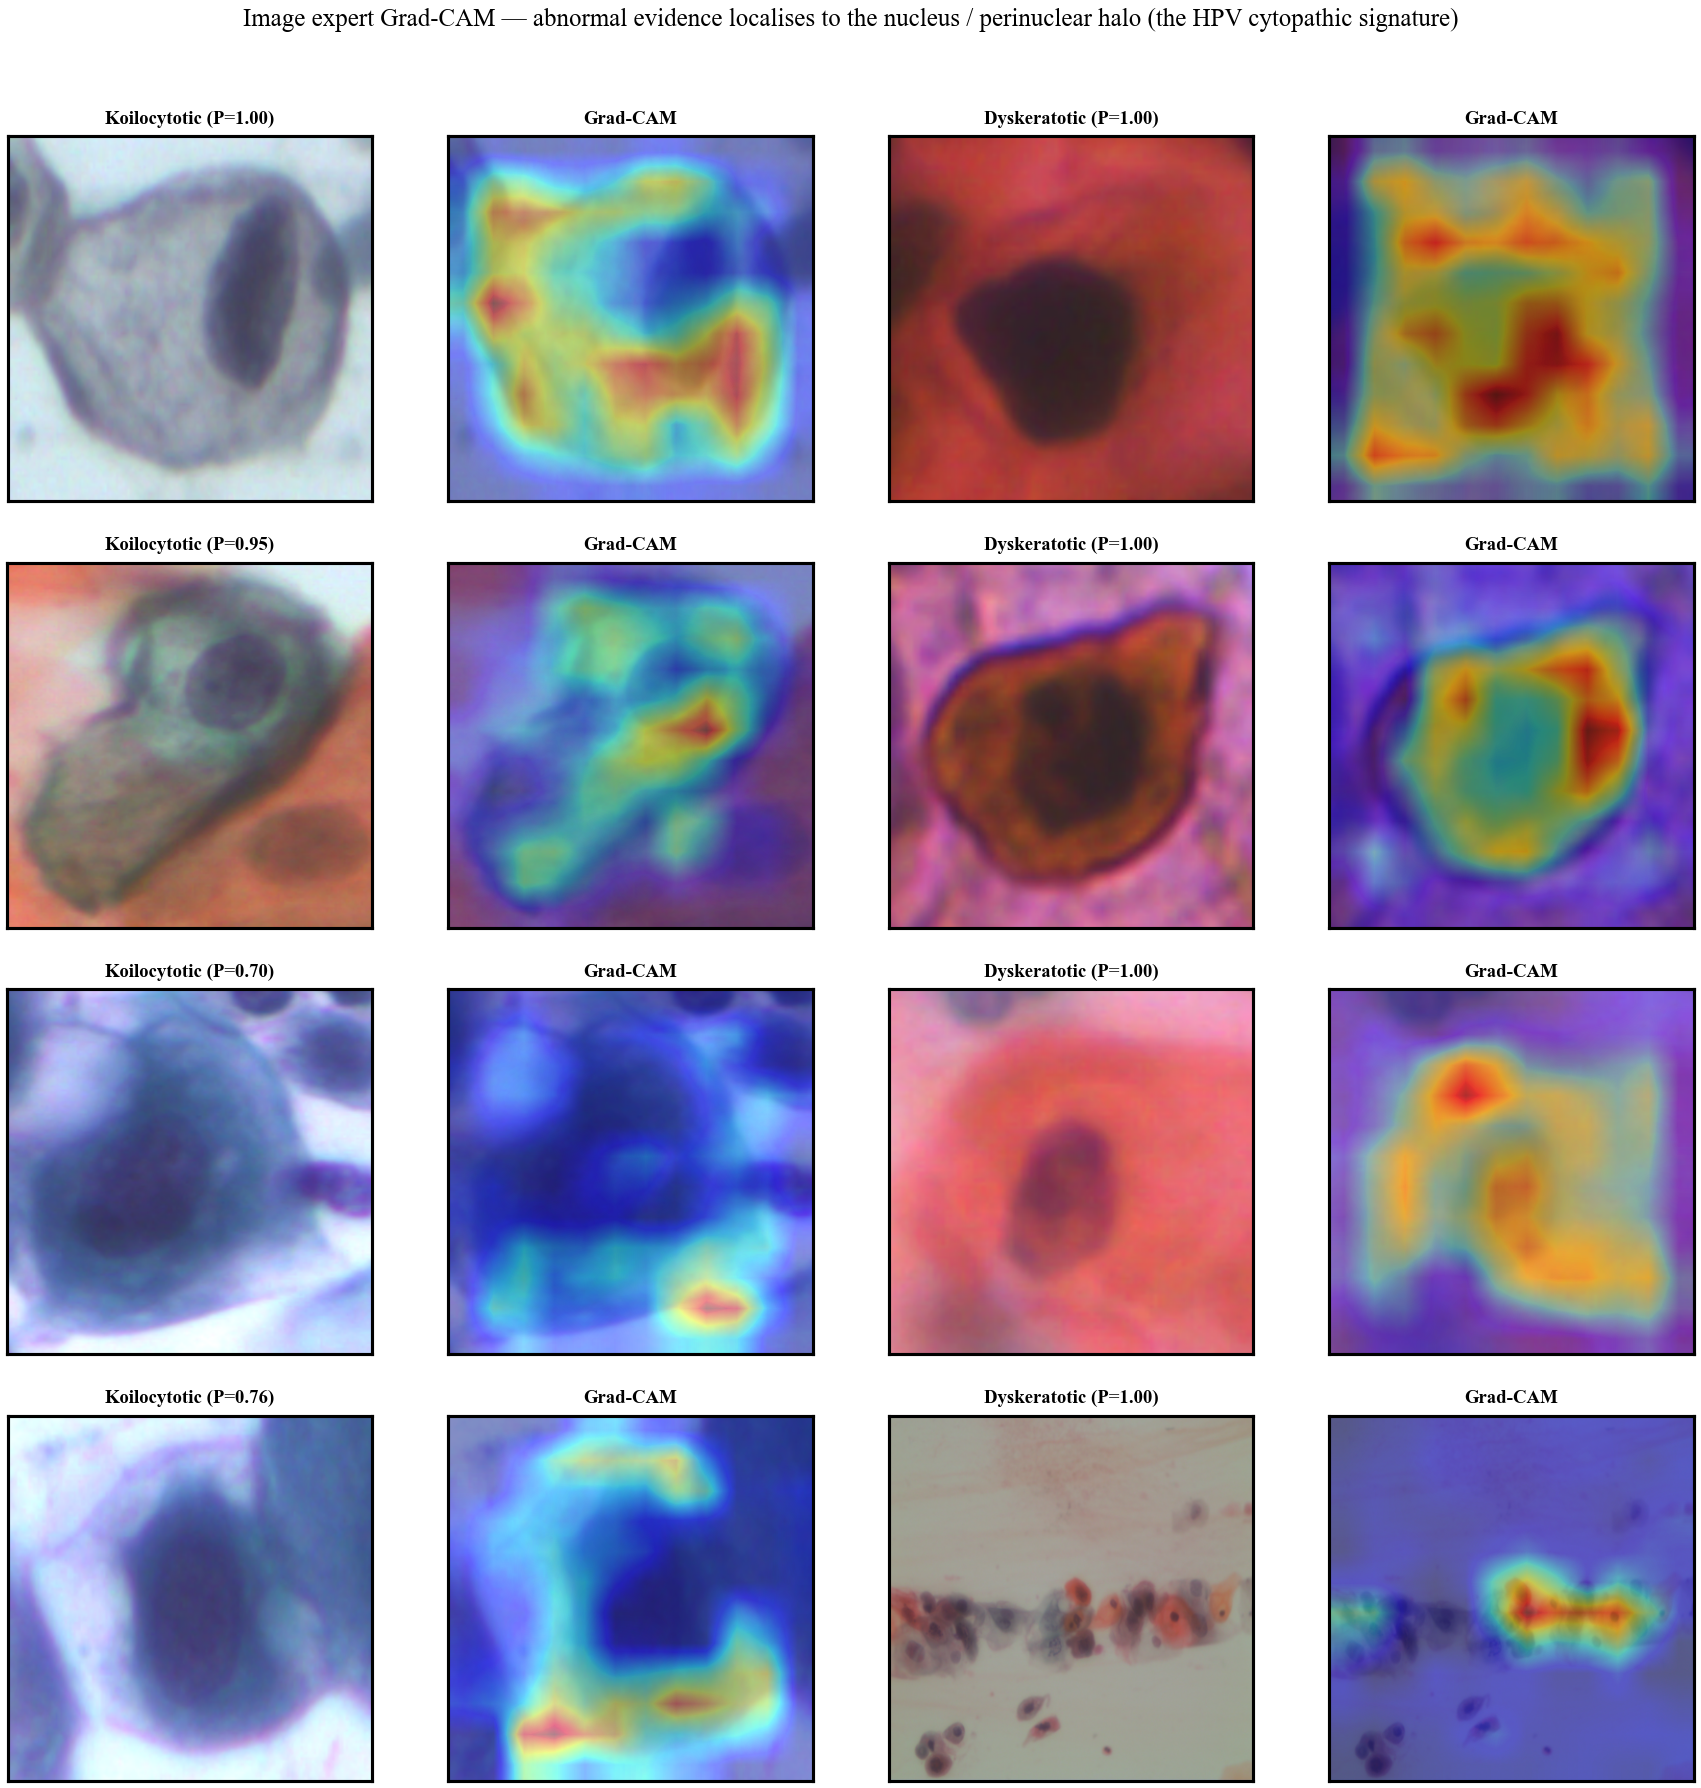
\includegraphics[width=\columnwidth]{figures/image_gradcam.png}
\caption{Grad-CAM on high-confidence Koilocytotic and Dyskeratotic cells: attribution concentrates on
nuclear/perinuclear regions.}
\Description{Grid of cells with Grad-CAM overlays.}
\label{fig:gradcam}
\end{figure}

\paragraph{Cross-dataset transfer.} Applied without re-training, AUROC on Herlev is $0.728$ and balanced
accuracy on APACC and HiCervix is $0.535$ and $0.562$ (Table~\ref{tab:img}; Herlev confusion matrix in
Figure~\ref{fig:cross}). Performance therefore varies substantially across collections, indicating marked
sensitivity to acquisition and population differences rather than uniform generalisation.

\begin{figure}[tb]\centering
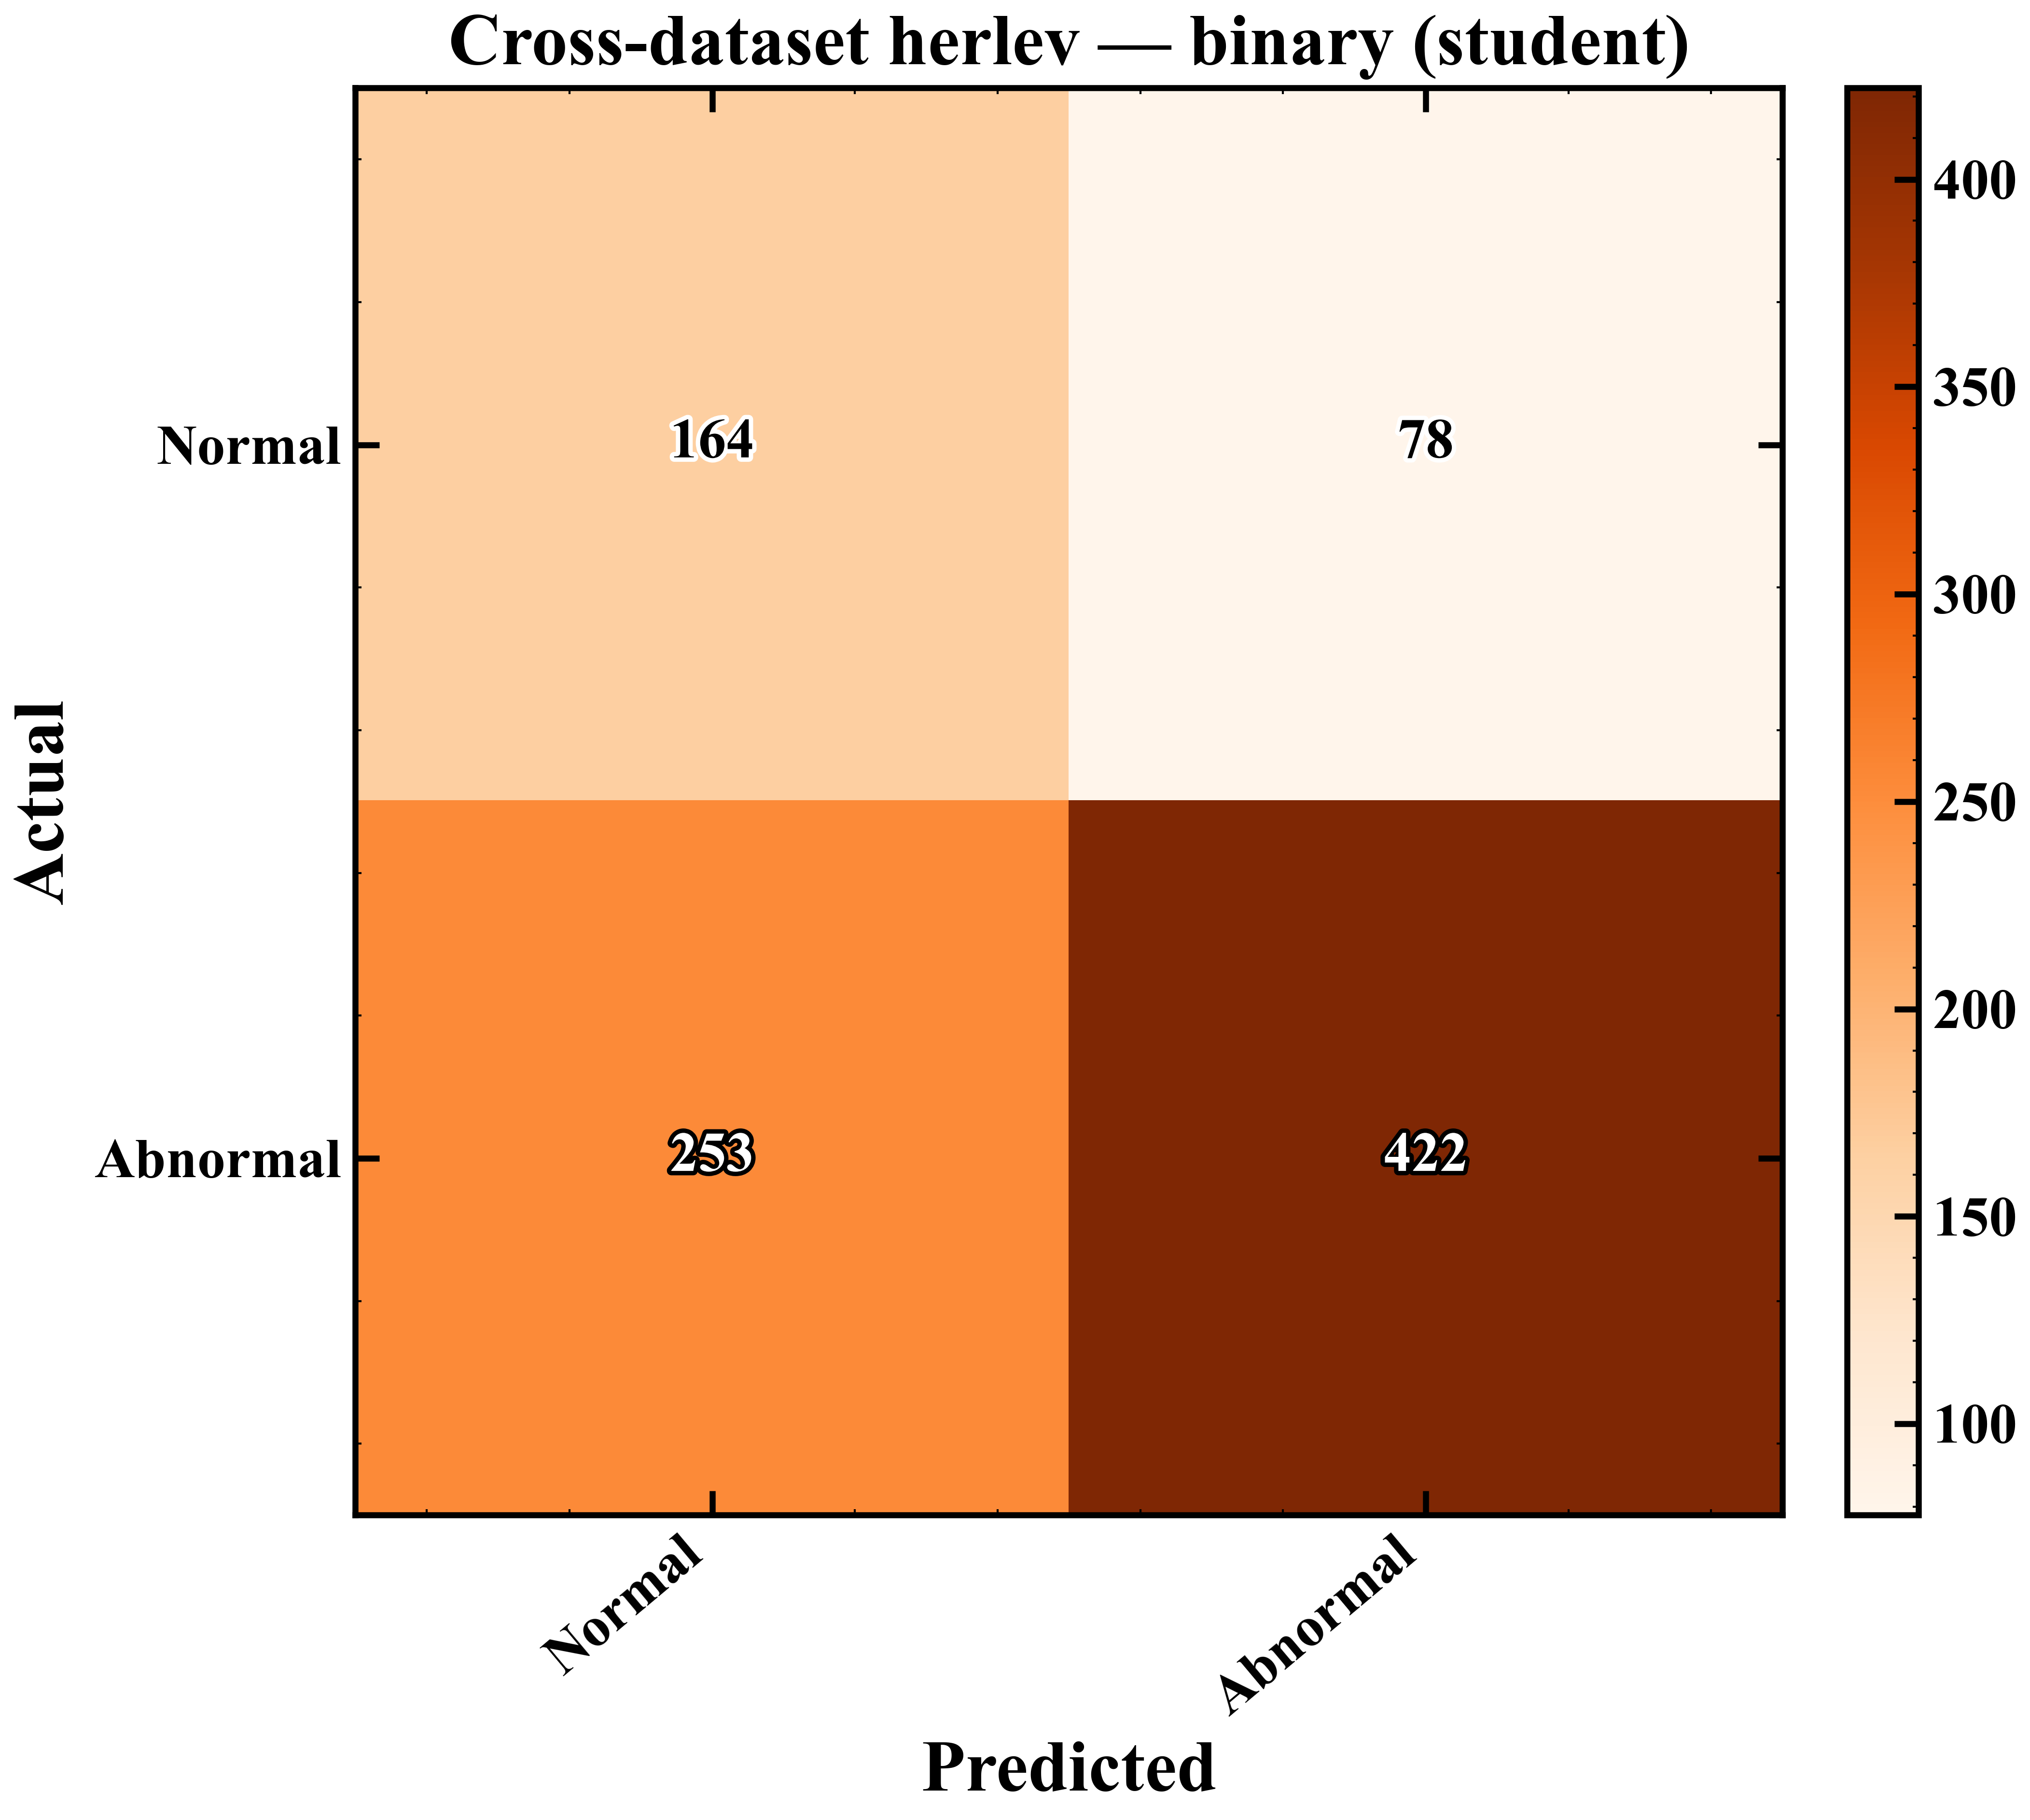
\includegraphics[width=0.66\columnwidth]{figures/cm_cross_herlev.png}
\caption{Binary (normal/abnormal) confusion matrix on the external Herlev dataset (AUROC $0.728$).}
\Description{Two-by-two confusion matrix.}
\label{fig:cross}
\end{figure}

%% ================= TABULAR EXPERT RESULTS =================
\subsection{HPV-risk expert}\label{sec:tabres}
\paragraph{Model comparison.} Among the five families (Figure~\ref{fig:tbake}, Table~\ref{tab:tab}) the tree
ensembles lead on AUROC; RandomForest is best, with $0.688$ AUROC and $0.721$ accuracy ($0.397$ F1, $0.423$
precision, $0.374$ recall) under $5$-fold cross-validation on the real cohort. Discrimination from
questionnaire data alone is modest but consistent across the tree families (AUROC $0.68$--$0.69$).

\begin{figure}[tb]\centering
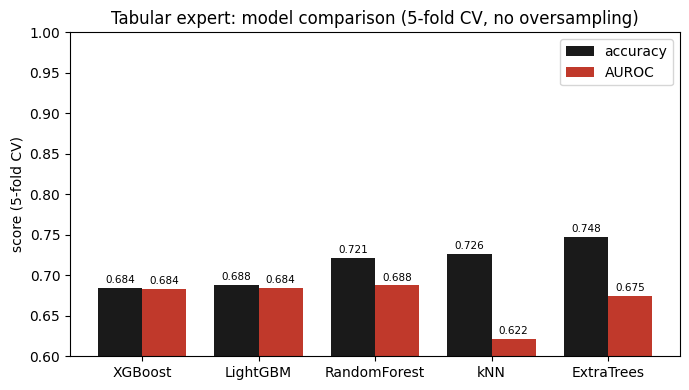
\includegraphics[width=\columnwidth]{figures/tabx_bakeoff.png}
\caption{HPV-risk model comparison (5-fold CV): accuracy and AUROC per classifier family.}
\Description{Grouped bar chart of accuracy and AUROC.}
\label{fig:tbake}
\end{figure}

\begin{table}[tb]\centering\footnotesize\setlength{\tabcolsep}{5pt}
\caption{HPV-risk expert on NHANES ($n=12{,}634$), 5-fold CV (class weights, no oversampling). RandomForest
obtains the highest AUROC.}
\label{tab:tab}
\begin{tabular}{@{}lccccc@{}}
\toprule
\textbf{Model} & \textbf{Acc} & \textbf{AUROC} & \textbf{F1} & \textbf{Prec} & \textbf{Rec}\\
\midrule
\textbf{RandomForest} & 0.721 & \textbf{0.688} & 0.397 & 0.423 & 0.374\\
LightGBM & 0.688 & 0.684 & 0.439 & 0.394 & 0.497\\
XGBoost & 0.684 & 0.684 & 0.444 & 0.391 & 0.514\\
ExtraTrees & 0.748 & 0.675 & 0.236 & 0.460 & 0.159\\
$k$-NN & 0.726 & 0.622 & 0.289 & 0.399 & 0.227\\
\bottomrule
\end{tabular}
\end{table}

\paragraph{Best-model evaluation.} For RandomForest, the confusion matrix, ROC, and precision--recall curves
(Figure~\ref{fig:teval}) give AUROC $0.688$; at the default $0.5$ threshold precision is $0.423$ and recall
$0.374$. From questionnaire inputs alone the model yields a modest but usable pre-test risk signal---helpful
for prioritising who to test rather than as a standalone diagnostic---and the operating point can be shifted
along the ROC/PR curves toward higher recall when used as a triage flag.

\begin{figure*}[t]\centering
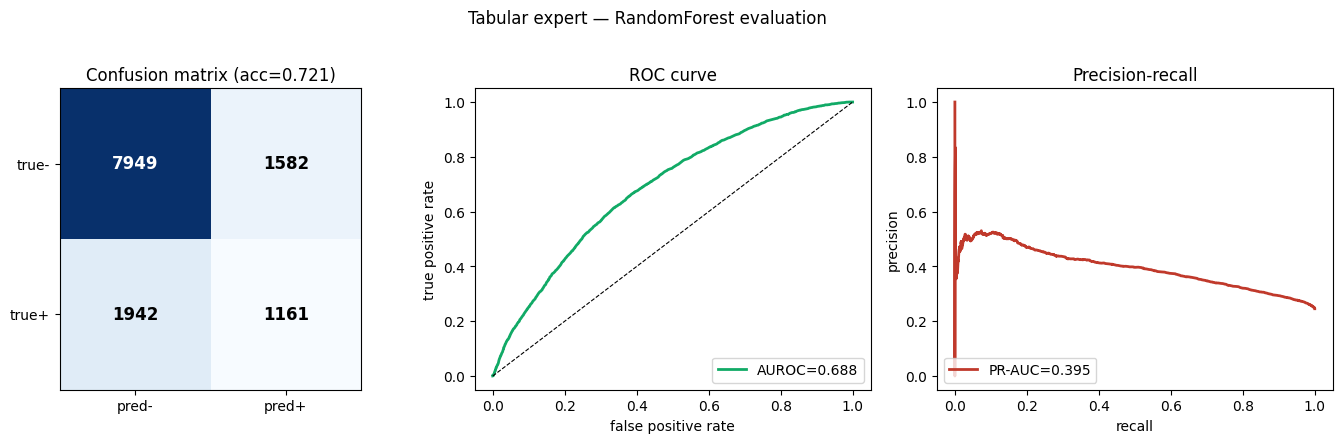
\includegraphics[width=0.92\textwidth]{figures/tabx_eval.png}
\caption{HPV-risk expert (RandomForest): confusion matrix (left), ROC (centre), precision--recall (right).}
\Description{Three-panel evaluation.}
\label{fig:teval}
\end{figure*}

\paragraph{Calibration and drivers.} After isotonic calibration the reliability curve follows the diagonal
(Figure~\ref{fig:trel}). Feature importance (Figure~\ref{fig:timp}) and SHAP attribution~\cite{lundberg2017shap}
(Figure~\ref{fig:tshap}) agree that behavioural-exposure variables---marital status, lifetime number of
partners, age, and the partner-acquisition rate---have the largest effect, in the directions expected from HPV
epidemiology, which supports that the model captures genuine risk structure rather than dataset artefacts.

\begin{figure}[tb]\centering
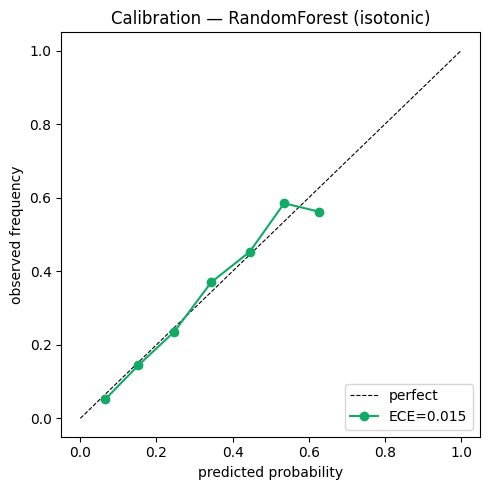
\includegraphics[width=0.7\columnwidth]{figures/tabx_reliability.png}
\caption{HPV-risk expert reliability diagram (isotonic-calibrated).}
\Description{Reliability curve near the diagonal.}
\label{fig:trel}
\end{figure}

\begin{figure}[tb]\centering
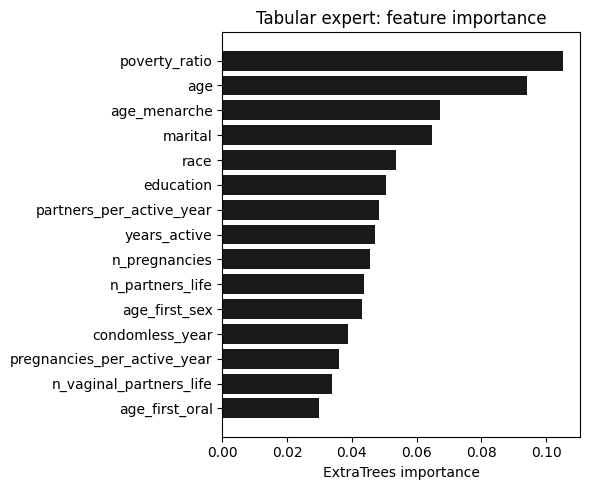
\includegraphics[width=0.82\columnwidth]{figures/tabx_importance.png}
\caption{HPV-risk expert feature importance (impurity-based, tree ensemble).}
\Description{Horizontal bar chart of feature importances.}
\label{fig:timp}
\end{figure}

\begin{figure}[tb]\centering
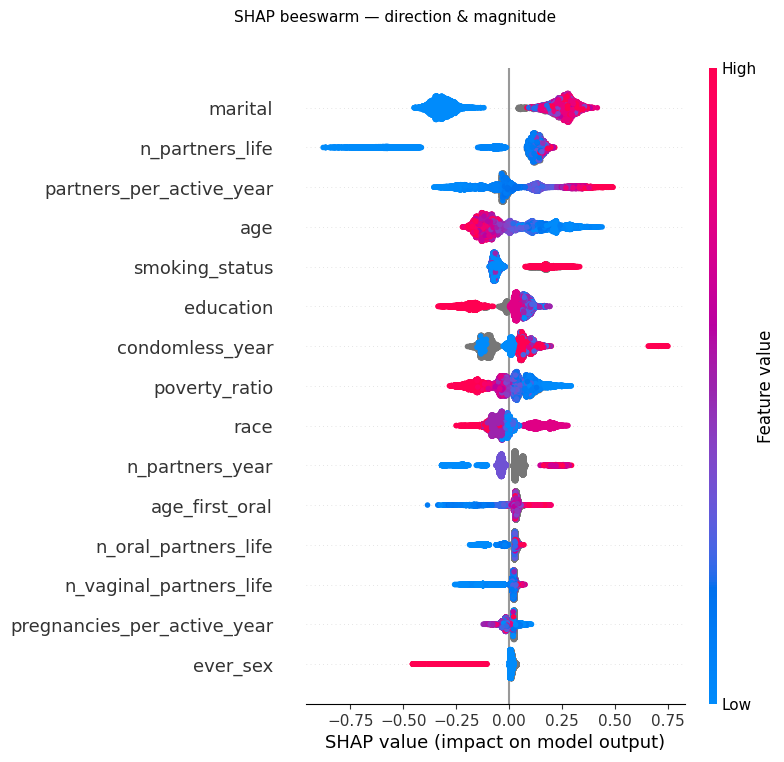
\includegraphics[width=\columnwidth]{figures/tabx_shap.png}
\caption{SHAP beeswarm for the HPV-risk expert (feature value in colour; horizontal position is the
contribution toward the positive class).}
\Description{SHAP beeswarm plot.}
\label{fig:tshap}
\end{figure}

%% ================= FUSED MODEL RESULTS =================
\subsection{Fused system}\label{sec:fusres}
\paragraph{Discrimination is not the point.} On a constructed deployment cohort the cytology expert reaches
$0.998$ AUROC and the HPV-risk expert $0.70$ (its $5$-fold value is $0.688$), and the fused output reaches
$0.993$ (Figures~\ref{fig:fmarg}--\ref{fig:froc})---essentially matching the stronger single expert. The fusion
therefore does \emph{not} increase discrimination over the stronger single expert---nor is it expected to. Its
purpose is to add complementary HPV-risk information, remain calibrated across deployment prevalences, and
operate under a missing modality (Table~\ref{tab:modes}).

\begin{figure}[tb]\centering
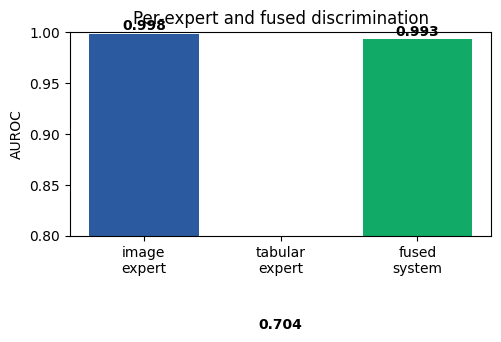
\includegraphics[width=0.72\columnwidth]{figures/fusx_marginals.png}
\caption{AUROC of each single expert and of the fused output on the constructed cohort.}
\Description{Bar chart of image, tabular, and fused AUROC.}
\label{fig:fmarg}
\end{figure}

\begin{figure}[tb]\centering
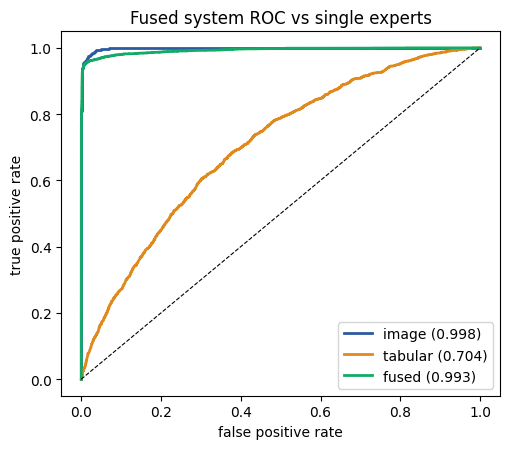
\includegraphics[width=0.72\columnwidth]{figures/fusx_roc.png}
\caption{ROC curves of the cytology expert, HPV-risk expert, and fused output.}
\Description{ROC curves.}
\label{fig:froc}
\end{figure}

\begin{table}[tb]\centering\footnotesize\setlength{\tabcolsep}{6pt}
\caption{Operating modes. The system runs whichever modality is present and returns the corresponding
calibrated output.}
\label{tab:modes}
\begin{tabular}{@{}lcc@{}}
\toprule
\textbf{Available input} & \textbf{Output} & \textbf{AUROC}\\
\midrule
image only & $p_{\mathrm{img}}$ (cytology) & 0.998\\
questionnaire only & $p_{\mathrm{tab}}$ (HPV-risk) & 0.688\\
both & $p_{\mathrm{fused}}$ (calibrated) & 0.993\\
\bottomrule
\end{tabular}
\end{table}

\paragraph{Calibration across prevalence (CO-PRIOR).} Without re-anchoring, calibration error grows as the
deployment prevalence $\tau$ departs from the training prevalence; with CO-PRIOR it is reduced substantially
across the tested range---for example ECE $0.21\!\to\!0.00$ at $\tau=0.02$ (Figure~\ref{fig:fcop}). This is the
main quantitative benefit of the fusion machinery.

\begin{figure}[tb]\centering
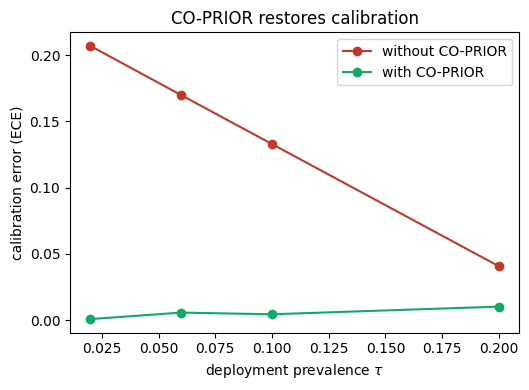
\includegraphics[width=0.78\columnwidth]{figures/fusx_coprior.png}
\caption{CO-PRIOR: expected calibration error versus deployment prevalence $\tau$, with and without prior
re-anchoring.}
\Description{Two ECE-versus-prevalence curves.}
\label{fig:fcop}
\end{figure}

\paragraph{Abstention coverage.} Split-conformal coverage is close to the target for the HPV-risk expert
($0.904$ at target $0.90$) and somewhat below target for the cytology expert ($0.855$ at target $0.90$;
Figure~\ref{fig:fcov}, Table~\ref{tab:fus}). The coverage guarantee is therefore approximately met for the
HPV-risk expert and close for the cytology expert at this level.

\begin{figure}[tb]\centering
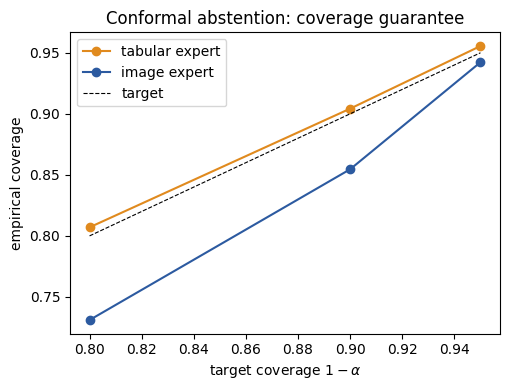
\includegraphics[width=0.72\columnwidth]{figures/fusx_coverage.png}
\caption{Split-conformal empirical coverage versus target $1-\alpha$ for each expert.}
\Description{Empirical-versus-target coverage lines.}
\label{fig:fcov}
\end{figure}

\begin{table}[tb]\centering\footnotesize\setlength{\tabcolsep}{5pt}
\caption{Fused-system summary. Fusion does not raise discrimination; its measured benefit is calibration
across prevalence.}
\label{tab:fus}
\begin{tabular}{@{}lc@{}}
\toprule
\textbf{Quantity} & \textbf{Value}\\
\midrule
Cytology expert AUROC & 0.998\\
HPV-risk expert AUROC & 0.688\\
Fused output AUROC & 0.993\\
Fused ECE & 0.043\\
CO-PRIOR ECE at $\tau=0.02$ & $0.21\!\to\!0.00$\\
Conformal coverage at target $0.90$ & 0.904 (HPV-risk) / 0.855 (cytology)\\
\bottomrule
\end{tabular}
\end{table}

%% =====================================================================
\section{Discussion}
The cytology expert performs strongly on its own endpoint ($0.998$ validation AUROC for cytological
abnormality) and the HPV-risk expert gives a modest but usable signal ($0.688$ cross-validated AUROC for
high-risk HPV)---and, importantly, each emits a calibrated probability. The fusion does not improve discrimination beyond the stronger expert, and we do not claim it
does; its role is to (i) reconcile the two differently-calibrated outputs onto one deployment-prevalence scale
(CO-PRIOR), (ii) keep the fused probability calibrated when the local disease rate differs from the training
population, and (iii) return the appropriate calibrated output when only one modality is available. Framed this
way, the value of CytoBridge is operational---combining heterogeneous, unpaired evidence with calibrated,
missing-modality behaviour---rather than a discrimination gain.

%% =====================================================================
\section{Limitations}\label{sec:limits}
\begin{itemize}
  \item \emph{No independent test set for the cytology expert.} The $0.966/0.998$ figures are validation-split,
    in-distribution numbers; a held-out or prospective test set would give a less optimistic estimate.
  \item \emph{Unpaired modalities.} No patient has both an image and a questionnaire, so the fused decision is
    analysed per expert and on a constructed cohort, not measured on real paired data.
  \item \emph{Domain shift.} External image performance drops markedly (Herlev $0.728$; APACC $0.535$;
    HiCervix $0.562$ balanced accuracy), so in-distribution results do not transfer uniformly.
\end{itemize}

%% =====================================================================
\section{Conclusion}
We asked whether independently trained cytology and questionnaire HPV-risk models can be combined at the
decision level to give calibrated, any-modality screening support without paired patient data. The two experts
reach $0.998$ (validation) and $0.688$ (cross-validation) AUROC on their respective endpoints. Combining them
with CO-PRIOR prior re-anchoring, an asymmetric combiner, and conformal abstention does not increase
discrimination beyond the stronger expert, but it keeps the fused probability calibrated across deployment
prevalences and lets the system operate when a modality is missing. The main open problems---an independent
and ideally paired test cohort, and the observed domain-shift sensitivity of the image model---are the natural
next steps toward clinical evaluation.

\bibliographystyle{ACM-Reference-Format}
\bibliography{refs}
\end{document}
